
\chapter{Stability of defection, optimisation of strategies and the limits of
       memory in the Prisoner's Dilemma.}\label{chapter:memory_one}


% Memory-one strategies are a set of Iterated Prisoner's Dilemma strategies
% that have been praised for their mathematical tractability and performance
% against single opponents. This manuscript investigates \textit{best
% response} memory-one strategies as a multidimensional
% optimisation problem. Though extortionate memory-one strategies have gained
% much attention, we demonstrate that best response memory-one strategies do not
% behave in an extortionate way, and moreover, for memory one strategies to be
% evolutionary robust they need to be able to behave in a forgiving way. We
% also provide evidence that memory-one strategies suffer from their limited
% memory in multi agent interactions and can be out performed by
% longer memory strategies.

% \section{Introduction}\label{section:introduction}

% The Prisoner's Dilemma (PD) is a two player game used in understanding the
% evolution of cooperative behaviour, formally introduced in~\cite{Flood1958}.
% Each player has two options, to cooperate (C) or to defect (D). The decisions
% are made simultaneously and independently. The normal form representation of the
% game is given by:

% \begin{equation}\label{equ:pd_definition}
%     S_p =
%     \begin{pmatrix}
%         R & S  \\
%         T & P
%     \end{pmatrix}
%     \quad
%     S_q =
%     \begin{pmatrix}
%         R & T  \\
%         S & P
%     \end{pmatrix}
% \end{equation}

% where \(S_p\) represents the utilities of the row player and \(S_q\) the
% utilities of the column player. The payoffs, \((R, P, S, T)\), are constrained
% by equations~(\ref{eq:pd_constrain_one}) and~(\ref{eq:pd_constrain_two}).
% Constraint~(\ref{eq:pd_constrain_one}) ensures that
% defection dominates cooperation and constraint~(\ref{eq:pd_constrain_two})
% ensures that there is a dilemma; the sum of the utilities for both players is
% better when both choose to cooperate. The most common values used in the literature are
% \((R, P, S, T) = (3, 1, 0, 5)\)~\cite{Axelrod1981}.


% \begin{equation}\label{eq:pd_constrain_one}
%     T > R > P > S
% \end{equation}

% \begin{equation}\label{eq:pd_constrain_two}
%     2R > T + S
% \end{equation}

% The PD is a one shot game, however, it is commonly studied in a manner where the
% history of the interactions matters. The repeated form of the game is called the
% Iterated Prisoner's Dilemma (IPD) and in the 1980s, following the work
% of~\cite{Axelrod1980a, Axelrod1980b} it attracted the attention of the
% scientific community. In~\cite{Axelrod1980a} and~\cite{Axelrod1980b}, the first
% well known computer tournaments of the IPD were performed. A total of 13 and 62
% strategies were submitted respectively in the form of computer code. The
% contestants competed against each other, a copy of themselves and a random
% strategy, and the winner was then decided on the average score achieved (not the
% total number of wins). The contestants were given access to the entire history
% of a match, however, how many turns of history a strategy would incorporate,
% referred to as the \textit{memory size} of a strategy, was a result of the
% particular strategic decisions made by the author. The winning strategy of both
% tournaments was a strategy called Tit for Tat and its success in both
% tournaments came as a surprise. Tit for Tat was a simple, forgiving strategy
% that opened each interaction by cooperation, and had won the tournament even
% though it never scored higher than that its direct opponent. Tit for Tat provided
% evidence that being nice can be advantageous and became the major paradigm for
% reciprocal altruism.

% Another trait of Tit for Tat is that it considers only the previous move of the
% opponent. These type of strategies are called \textit{reactive} \cite{Nowak1989}
% and are a subset of so called \textit{memory-one} strategies, which incorporate
% both players' latests moves. Memory-one strategies have been
% studied thoroughly in the literature~\cite{Nowak1990, Nowak1993}, however, they have gained
% most of their attention when a certain subset of memory-one strategies was
% introduced in~\cite{Press2012}, the zero-determinants. In~\cite{Stewart2012} it
% was stated that ``Press and Dyson have fundamentally changed the viewpoint on
% the Prisoner's Dilemma''.
% Zero-determinants are a special case of memory-one and extortionate
% strategies. They choose their actions so that a linear relationship is forced
% between the players' score ensuring that they will always
% receive at least as much as their opponents. Zero-determinants are
% indeed mathematically unique and are proven to be robust in pairwise
% interactions, however, their true effectiveness in tournaments and
% evolutionary dynamics has been questioned~\cite{Adami2013, Hilbe2013b,
% Hilbe2013, Hilbe2015, Knight2018, Lee2015}.

% In a similar fashion to~\cite{Press2012} the purpose of this work is to consider
% a given memory-one strategy; however, whilst~\cite{Press2012} found a way for a
% player to manipulate a given opponent, this work will consider a
% multidimensional optimisation approach to identify the best response to a given
% group of opponents. In particular, this work presents a compact method of
% identifying the best response memory-one strategy against a given set of
% opponents, and evaluates whether it behaves extortionately, similar to
% zero-determinants. Further theoretical and empirical results of this work
% include:

% \begin{enumerate}
%     \item The conditions that ensure a best response memory-one strategy evolutionary
%     robust.
%     \item A well designed framework that allows the comparison of an optimal
%           memory one strategy and a more complex strategy which has a larger
%           memory and was obtained through reinforcement learning
%           techniques~\cite{Harper2017}.
%     \item An identification of conditions for which defection is known to be
%     stable; thus identifying environments where cooperation will not
%     occur.
% \end{enumerate}

% \section{The utility}\label{section:utility}

% One specific advantage of memory-one strategies is their mathematical
% tractability. They can be represented completely as an element of \(\R^{4}_{[0, 1]}\). This
% originates from~\cite{Nowak1989} where it is stated that if a strategy is
% concerned with only the outcome of a single turn then there are four possible
% `states' the strategy could be in;

% \begin{itemize}
%     \item both players cooperated, denoted as \(CC\)
%     \item first players cooperated whilst the second player defected, denoted as \(CD\)
%     \item first players defected whilst the second player cooperated, denoted as \(DC\)
%     \item both players defected, denoted as \(DD\)
% \end{itemize}

% Therefore, a memory-one strategy can be denoted by the probability vector of
% cooperating after each of these states; \(p=(p_1, p_2, p_3, p_4) \in \R_{[0,1]}
% ^ 4\).

% In~\cite{Nowak1989} it was shown that it is not necessary to simulate the play
% of a strategy $p$ against a memory-one opponent $q$. Rather this exact behaviour
% can be modelled as a stochastic process, and more specifically as a Markov chain
% (Figure~\ref{fig:markov_chain}) whose corresponding transition matrix \(M\) is
% given by (\ref{eq:transition_matrix}). The long run steady state probability
% vector \(v\), which is the solution to \(v M = v\), can be
% combined with the payoff matrices of (\ref{equ:pd_definition}) to give the expected
% payoffs for each player. More specifically, the utility for a memory-one
% strategy \(p\) against an opponent \(q\), denoted as \(u_q(p)\), is given by
% (\ref{eq:press_dyson_utility}).

% \begin{figure}
%     \centering
%     \includestandalone[width=.35\textwidth]{src/chapters/05/paper/Memory-size-in-the-prisoners-dilemma/tex/markov_chain}
%     \caption{Markov Chain}
%     \label{fig:markov_chain}
% \end{figure}

% \begin{equation}\label{eq:transition_matrix}
%     M = \left[\begin{matrix}p_{1} q_{1} & p_{1} \left(- q_{1} + 1\right) & q_{1} \left(- p_{1} + 1\right) & \left(- p_{1} + 1\right) \left(- q_{1} + 1\right)\\p_{2} q_{3} & p_{2} \left(- q_{3} + 1\right) & q_{3} \left(- p_{2} + 1\right) & \left(- p_{2} + 1\right) \left(- q_{3} + 1\right)\\p_{3} q_{2} & p_{3} \left(- q_{2} + 1\right) & q_{2} \left(- p_{3} + 1\right) & \left(- p_{3} + 1\right) \left(- q_{2} + 1\right)\\p_{4} q_{4} & p_{4} \left(- q_{4} + 1\right) & q_{4} \left(- p_{4} + 1\right) & \left(- p_{4} + 1\right) \left(- q_{4} + 1\right)\end{matrix}\right]
% \end{equation}


% \begin{equation}\label{eq:press_dyson_utility}
%     u_q(p) = v \cdot (R, S, T, P).
% \end{equation}

% This manuscript has explored the form of \(u_q(p)\), to the authors knowledge no
% previous work has done this, and it proves that \(u_q(p)\) is given by a ratio
% of two quadratic forms~\cite{kepner2011},
% Theorem~\ref{theorem:quadratic_form_u}.

% \begin{theorem}\label{theorem:quadratic_form_u}
%     The expected utility of a memory-one strategy \(p\in\mathbb{R}_{[0,1]}^4\)
%     against a memory-one opponent \(q\in\mathbb{R}_{[0,1]}^4\), denoted
%     as \(u_q(p)\), can be written as a ratio of two quadratic forms:

%     \begin{equation}\label{eq:optimisation_quadratic}
%     u_q(p) = \frac{\frac{1}{2}pQp^T + cp + a}
%                 {\frac{1}{2}p\bar{Q}p^T + \bar{c}p + \bar{a}},
%     \end{equation}
%     where \(Q, \bar{Q}\) \(\in \R^{4\times4}\) are square matrices defined by the
%     transition probabilities of the opponent \(q_1, q_2, q_3, q_4\) as follows:

%     \begin{center}
%     \begin{equation}
%     \resizebox{0.9\linewidth}{!}{\arraycolsep=2.5pt%
%     \boldmath\(
%     Q = \left[\begin{matrix}0 & - \left(q_{1} - q_{3}\right) \left(q_{2} - 5 q_{4} - 1\right) & q_{3} \left(q_{1} - q_{2}\right) & - 5 q_{3} \left(q_{1} - q_{4}\right)\\- \left(q_{1} - q_{3}\right) \left(q_{2} - 5 q_{4} - 1\right) & 0 & \left(q_{2} - q_{3}\right) \left(q_{1} - 3 q_{4} - 1\right) & \left(q_{3} - q_{4}\right) \left(5 q_{1} - 3 q_{2} - 2\right)\\q_{3} \left(q_{1} - q_{2}\right) & \left(q_{2} - q_{3}\right) \left(q_{1} - 3 q_{4} - 1\right) & 0 & 3 q_{3} \left(q_{2} - q_{4}\right)\\- 5 q_{3} \left(q_{1} - q_{4}\right) & \left(q_{3} - q_{4}\right) \left(5 q_{1} - 3 q_{2} - 2\right) & 3 q_{3} \left(q_{2} - q_{4}\right) & 0\end{matrix}\right]\)},
%     \end{equation}
%     \begin{equation}\label{eq:q_bar_matrix}
%     \resizebox{0.8\linewidth}{!}{\arraycolsep=2.5pt%
%     \boldmath\(
%     \bar{Q} =  \left[\begin{matrix}0 & - \left(q_{1} - q_{3}\right) \left(q_{2} - q_{4} - 1\right) & \left(q_{1} - q_{2}\right) \left(q_{3} - q_{4}\right) & \left(q_{1} - q_{4}\right) \left(q_{2} - q_{3} - 1\right)\\- \left(q_{1} - q_{3}\right) \left(q_{2} - q_{4} - 1\right) & 0 & \left(q_{2} - q_{3}\right) \left(q_{1} - q_{4} - 1\right) & \left(q_{1} - q_{2}\right) \left(q_{3} - q_{4}\right)\\\left(q_{1} - q_{2}\right) \left(q_{3} - q_{4}\right) & \left(q_{2} - q_{3}\right) \left(q_{1} - q_{4} - 1\right) & 0 & - \left(q_{2} - q_{4}\right) \left(q_{1} - q_{3} - 1\right)\\\left(q_{1} - q_{4}\right) \left(q_{2} - q_{3} - 1\right) & \left(q_{1} - q_{2}\right) \left(q_{3} - q_{4}\right) & - \left(q_{2} - q_{4}\right) \left(q_{1} - q_{3} - 1\right) & 0\end{matrix}\right]\)}.
%     \end{equation}
%     \end{center}

%     \(c \text{ and } \bar{c}\) \(\in \R^{4 \times 1}\) are similarly defined by:

%     \begin{equation}\label{eq:q_matrix_numerator}
%     \resizebox{0.3\linewidth}{!}{\arraycolsep=2.5pt%
%     \boldmath\(c = \left[\begin{matrix}q_{1} \left(q_{2} - 5 q_{4} - 1\right)\\- \left(q_{3} - 1\right) \left(q_{2} - 5 q_{4} - 1\right)\\- q_{1} q_{2} + q_{2} q_{3} + 3 q_{2} q_{4} + q_{2} - q_{3}\\5 q_{1} q_{4} - 3 q_{2} q_{4} - 5 q_{3} q_{4} + 5 q_{3} - 2 q_{4}\end{matrix}\right]\),}
%     \end{equation}
%     \begin{equation}\label{eq:q_matrix_denominator}
%     \resizebox{0.3\linewidth}{!}{\arraycolsep=2.5pt%
%     \boldmath\(\bar{c} = \left[\begin{matrix}q_{1} \left(q_{2} - q_{4} - 1\right)\\- \left(q_{3} - 1\right) \left(q_{2} - q_{4} - 1\right)\\- q_{1} q_{2} + q_{2} q_{3} + q_{2} - q_{3} + q_{4}\\q_{1} q_{4} - q_{2} - q_{3} q_{4} + q_{3} - q_{4} + 1\end{matrix}\right]\),
%     }
%     \end{equation}
%     and the constant terms \(a, \bar{a}\) are defined as \(a = - q_{2} + 5 q_{4} + 1\) and
%     \(\bar{a} = - q_{2} + q_{4} + 1\).
% \end{theorem}

% The proof of Theorem~\ref{theorem:quadratic_form_u} is given in
% Appendix~\ref{appendix:proof_theorem_one}. Furthermore, numerical simulations
% have been carried out to validate the result. The simulated utility, which is
% denoted as \(U_q(p)\), has been calculated using~\cite{axelrodproject} an open
% source research framework for the study of the IPD (\cite{axelrodproject} is
% described in~\cite{Knight2016}). For smoothing the simulated results the utility
% has been estimated in a tournament of 500 turns and 200 repetitions.
% Figure~\ref{fig:analytical_simulated} shows two examples demonstrating that the
% formulation of Theorem~\ref{theorem:quadratic_form_u} successfully captures the
% simulated behaviour.

% The source code used in this manuscript has been written in a sustainable manner.
% It is open source (\url{https://github.com/Nikoleta-v3/Memory-size-in-the-prisoners-dilemma})
% and tested which ensures the validity of the results. It has also been archived
% and can be found at.
% %TODO archive software

% \begin{figure}[!htbp]
%     \begin{center}
%         \begin{subfigure}{0.45\textwidth}
%             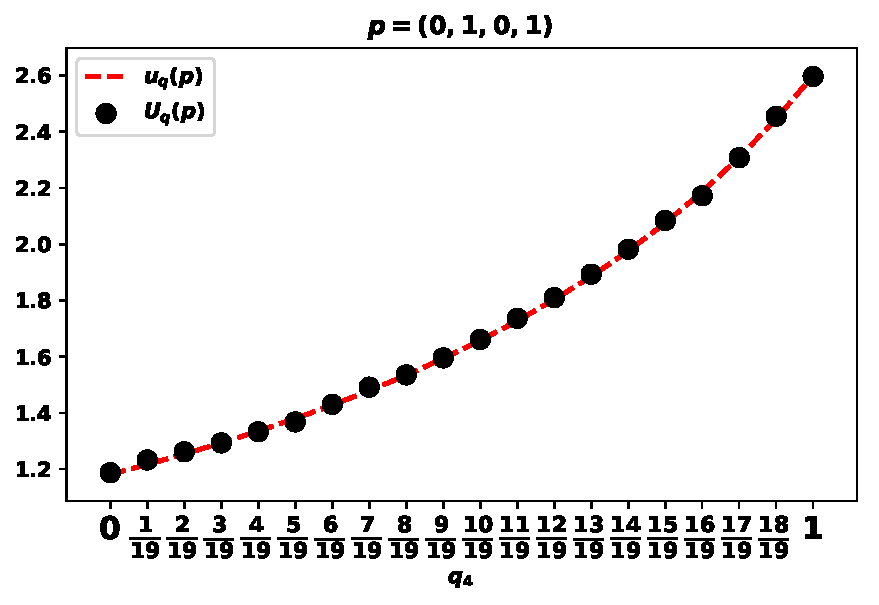
\includegraphics[width=\linewidth]{src/chapters/05/paper/Memory-size-in-the-prisoners-dilemma/img/validation_against_player_one.pdf}
%         \end{subfigure}
%         \begin{subfigure}{0.45\textwidth}
%             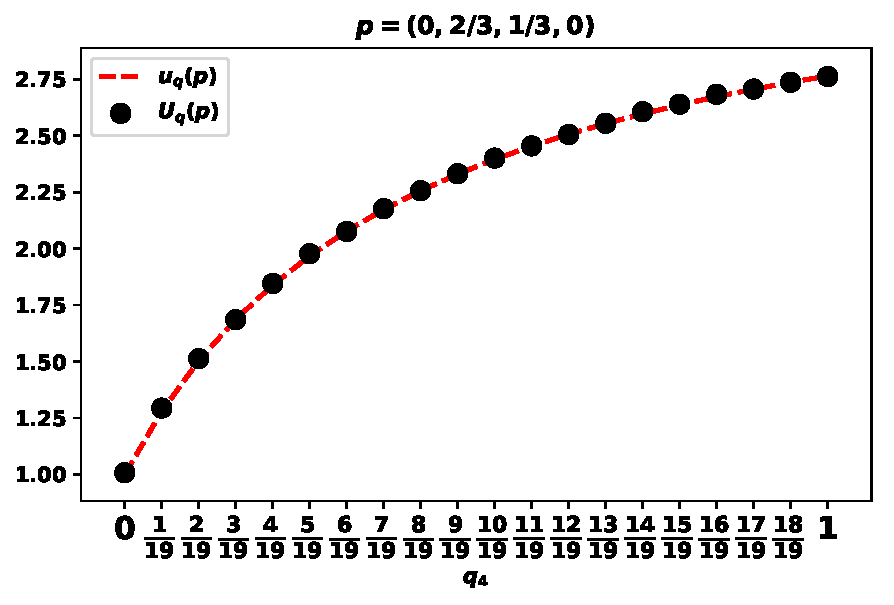
\includegraphics[width=\linewidth]{src/chapters/05/paper/Memory-size-in-the-prisoners-dilemma/img/validation_against_player_two.pdf}
%         \end{subfigure}
%     \end{center}
%     \caption{Simulated and empirical utilities for \(p = (0, 1, 0, 1)\)
%     and \(p = (0, \frac{2}{3}, \frac{1}{3}, 0)\) against \((\frac{1}{3}, \frac{1}{3}, \frac{1}{3}, q_4)\) for
%     \(q_4 \in \{0,  \frac{1}{19}, \frac{2}{19}, \dots, \frac{18}{19}, 1\}\).
%     \(u_q(p)\) is the theoretic value given in Theorem~\ref{theorem:quadratic_form_u},
%     and \(U_q(p)\) is simulated numerically.}
%     \label{fig:analytical_simulated}
% \end{figure}

% Theorem~\ref{theorem:quadratic_form_u} can be extended to consider multiple
% opponents. The IPD is commonly studied in tournaments and/or Moran Processes
% where a strategy interacts with a number of opponents. The payoff of a player in
% such interactions is given by the average payoff the player received against
% each opponent. More specifically the expected utility of a memory-one strategy
% against a \(N\) number of opponents is given by
% Theorem~\ref{theorem:tournament_utility}.

% \begin{theorem}\label{theorem:tournament_utility}
%     The expected utility of a memory-one strategy \(p\in\mathbb{R}_{[0,1]}^4\)
%     against a group of opponents \(q^{(1)}, q^{(2)}, \dots, q^{(N)}\), denoted
%     as \(\frac{1}{N} \sum\limits_{i=1} ^ {N} {u_q}^{(i)} (p)\), is given by:

%     \begin{equation}\label{eq:tournament_utility}
%         \frac{1}{N} \sum\limits_{i=1} ^ {N} {u_q}^{(i)} (p) = \frac{1}{N}
%         \frac{\sum\limits_{i=1} ^ {N} (\frac{1}{2} pQ^{(i)} p^T + c^{(i)} p + a^ {(i)})
%         \prod\limits_{\tiny\begin{array}{l} j=1 \\ j \neq i \end{array}} ^
%         N (\frac{1}{2} p\bar{Q}^{(j)} p^T + \bar{c}^{(j)} p + \bar{a}^ {(j)})}
%         {\prod\limits_{i=1} ^ N (\frac{1}{2} p\bar{Q}^{(i)} p^T + \bar{c}^{(i)} p + \bar{a}^ {(i)})}.
%     \end{equation}
% \end{theorem}

% The proof of Theorem~\ref{theorem:tournament_utility} is a straightforward algebraic
% manipulation.

% Similar to the previous result, the formulation of
% Theorem~\ref{theorem:tournament_utility} is validated using numerical
% simulations where the 10 memory-one strategies described in~\cite{Stewart2012}
% have been used as the opponents. Figure~\ref{fig:stewart_plotkin_results} shows
% that the simulated behaviour has been captured successfully.

% \begin{figure}[!htbp]
%     \begin{center}
%     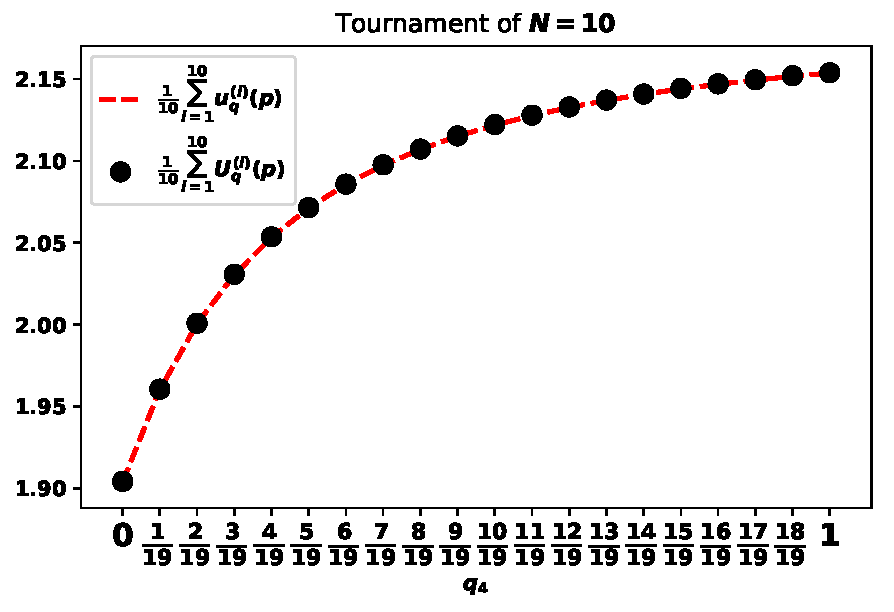
\includegraphics[width=.5\linewidth]{src/chapters/05/paper/Memory-size-in-the-prisoners-dilemma/img/Stewart_tournament_results.pdf}
%     \caption{The utilities of memory-one strategies \((\frac{1}{3}, \frac{1}{3}, \frac{1}{3}, p_4)\) for
%     \(p_4 \in \{0,  \frac{1}{19}, \frac{2}{19}, \dots, \frac{18}{19}, 1\}\)
%     against the 10 memory-one strategies described in~\cite{Stewart2012}.
%     \(\frac{1}{10} \sum^{10}_{i=1} u_q^{(i)}(p)\) is the theoretic value given in
%     Theorem~\ref{theorem:quadratic_form_u},
%     and \(\frac{1}{10} \sum^{10}_{i=1} U_q^{(i)}(p)\) is simulated numerically.}
%     \label{fig:stewart_plotkin_results}
%     \end{center}
% \end{figure}

% The list of strategies from~\cite{Stewart2012} was also used to check whether
% the utility against a group of strategies could be captured by the utility
% against the mean opponent. Thus whether condition (\ref{eq:condition}) holds.
% However condition~(\ref{eq:condition}) fails, as shown in
% Figure~\ref{fig:hypothesis}.

% \begin{equation}\label{eq:condition}
%     \frac{1}{N} \sum_{i=1} ^ {N} {u_q}^{(i)} (p) = u_{\frac {1}{N} \sum\limits_{i=1} ^ N q^{(i)}}(p),
% \end{equation}

% \begin{figure}[!htbp]
%     \begin{center}
%     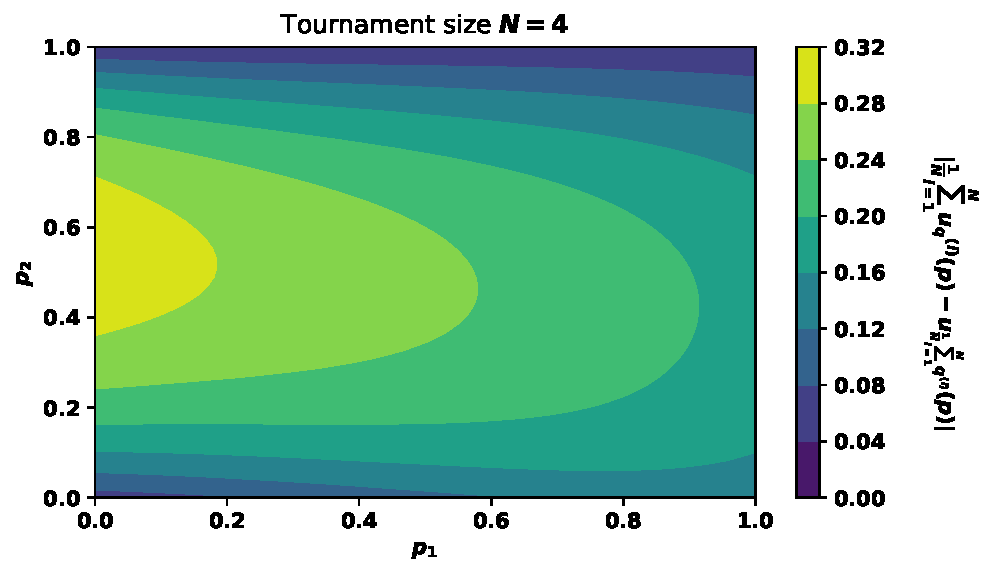
\includegraphics[width=.5\linewidth]{src/chapters/05/paper/Memory-size-in-the-prisoners-dilemma/img/mean_vs_average_heatmap.pdf}
%     \end{center}
%     \caption{The difference between the average utility against the opponents
%     from~\cite{Stewart2012} and the utility against the average player of the
%     strategies in~\cite{Stewart2012} of a player \(p=(p_1, p_2, p_1, p_2)\). A
%     positive difference indicates that condition (\ref{eq:condition}) does not
%     hold.}
%     \label{fig:hypothesis}
% \end{figure}

% Theorem~\ref{theorem:tournament_utility} which allows for the utility of a
% memory-one strategy against any number of opponents to be estimated without
% simulating the interactions is the main result used in this manuscript. In
% Section~\ref{section:best_response_mem_one} it is used to  define best response
% memory-one strategies and explore the conditions under which defection dominates
% cooperation.

% \section{Best responses to memory-one players}\label{section:best_response_mem_one}

% This section focuses on best responses and more specifically \textit{memory-one
% best response} strategies. A \textit{best response} is a strategy which
% corresponds to the most favourable outcome~\cite{Tadelis2013}, thus a memory-one
% best response to a set of opponents \(q^{(1)}, q^{(2)}, \dots, q^{(N)}\) corresponds to a strategy \(p^*\) for which
% (\ref{eq:tournament_utility}) is maximised. This is considered as a multi
% dimensional optimisation problem given by:

% \begin{equation}\label{eq:mo_tournament_optimisation}
%     \begin{aligned}
%     \max_p: & \ \sum_{i=1} ^ {N} {u_q}^{(i)} (p)
%     \\
%     \text{such that}: & \ p \in \R_{[0, 1]}
%     \end{aligned}
% \end{equation}

% Optimising this particular ratio of quadratic forms is not trivial. It can be
% verified empirically for the case of a single opponent that there exists at least
% one point for which the definition of concavity does not hold, see Appendix~\ref{appendix:non_concave}
% for an example. Some results are
% known for non concave ratios of quadratic forms~\cite{Beck2009, Hongyan2014},
% however, in these works it is assumed that either both the numerator and the
% denominator of the fractional problem are concave or that the denominator is
% greater than zero which in this case are not true
% (as seen in Theorem~\ref{theorem:concavity}).

% \begin{theorem}\label{theorem:concavity}
%     The utility of a player \(p\) against an opponent \(q\), \(u_q (p)\), given
%     by (\ref{eq:optimisation_quadratic}), is not concave. Furthermore neither
%     the numerator or the denominator of (\ref{eq:optimisation_quadratic}), are
%     concave or strictly greater than zero.
% \end{theorem}

% Proof is given in Appendix~\ref{appendix:proof_theorem_three}.

% The non concavity of \(u(p)\) indicates multiple local optimal points. The
% approach taken here is to introduce a compact way of constructing the candidate
% set of all local optimal points, and evaluating which corresponds to the best response
% strategy (maximises (\ref{eq:tournament_utility})).

% The problem considered is bounded because \(p \in \R^4_{[0, 1]}\).
% Therefore, the candidate solutions will exist either at the boundaries of the
% feasible solution space, or within that space (the methods of Lagrange
% Multipliers~\cite{bertsekas2014} and Karush-Kuhn-Tucker
% conditions~\cite{Giorgi2016} are based on this). This approach allow us to
% define the best response memory-one strategy to a group of opponents in the
% following Lemma:

% \begin{lemma}\label{lemma:memone_group_best_response}

%     The optimal behaviour of a memory-one strategy player
%     \(p^* \in \R_{[0, 1]} ^ 4\)
%     against a set of \(N\) opponents \(\{q^{(1)}, q^{(2)}, \dots, q^{(N)} \}\)
%     for \(q^{(i)} \in \R_{[0, 1]} ^ 4\) is given by:

%     \[p^* = \textnormal{argmax}\sum\limits_{i=1} ^ N  u_q(p), \ p \in S_q.\]

%     The set \(S_q\) is defined as all the possible combinations of:

%     \begin{equation}\label{eq:s_q_set}
%         S_q =
%         \left\{p \in \mathbb{R} ^ 4 \left|
%             \begin{aligned}
%                 \bullet\quad p_j \in \{0, 1\} & \quad \text{and} \quad \frac{d}{dp_k} 
%                 \sum\limits_{i=1} ^ N  u_q^{(i)}(p) = 0
%                 \quad \text{for all} \quad j \in J \quad \&  \quad k \in K  \quad \text{for all} \quad J, K \\
%                 & \quad \text{where} \quad J \cap K = \O \quad
%                 \text{and} \quad J \cup K = \{1, 2, 3, 4\}.\\
%                 \bullet\quad  p \in \{0, 1\} ^ 4
%             \end{aligned}\right.
%         \right\}.
%     \end{equation}
% \end{lemma}

% The proof is given in Appendix~\ref{appendix:proof_lemma_four}.

% Note that there is no immediate way to find the zeros of \(\frac{d}{dp} \sum\limits_{i=1} ^ N  u_q(p)\);

% {\small
% \begin{align}\label{eq:mo_tournament_derivative}
%     \frac{d}{dp} \sum\limits_{i=1} ^ {N} {u_q}^{(i)} (p) & = \nonumber \\
%     & =  \displaystyle\sum\limits_{i=1} ^ {N}
%     \frac{\left(pQ^{(i)} + c^{(i)}\right) \left(\frac{1}{2} p\bar{Q}^{(i)} p^T + \bar{c}^{(i)} p + \bar{a}^ {(i)}\right)
%     - \left(p\bar{Q}^{(i)} + \bar{c}^{(i)}\right) \left(\frac{1}{2} pQ^{(i)} p^T + c^{(i)} p + a^ {(i)}\right)}
%     {\left(\frac{1}{2} p\bar{Q}^{(i)} p^T + \bar{c}^{(i)} p + \bar{a}^ {(i)}\right)^ 2}
% \end{align}
% }

% For \(\frac{d}{dp} \sum\limits_{i=1} ^ N  u_q(p)\) to equal zero then:

% {\scriptsize
% \begin{align}\label{eq:polynomials_roots}
%     \displaystyle\sum\limits_{i=1} ^ {N} \left(
%     \left(pQ^{(i)} + c^{(i)}\right) \left(\frac{1}{2} p\bar{Q}^{(i)} p^T + \bar{c}^{(i)} p + \bar{a}^ {(i)}\right)
%     - \left(p\bar{Q}^{(i)} + \bar{c}^{(i)}\right) \left(\frac{1}{2} pQ^{(i)} p^T + c^{(i)} p + a^ {(i)}\right)\right)
%     &= 0, \quad {while} \\
%     \displaystyle\sum\limits_{i=1} ^ {N} \frac{1}{2} p\bar{Q}^{(i)} p^T + \bar{c}^{(i)} p + \bar{a}^ {(i)} &\neq 0.
% \end{align}}

% Finding best response memory-one strategies, more specifically constructing the
% subset \(S_q\), can be done analytically. The points for any or all of \(p_i \in
% \{0, 1\}\) for \(i \in \{1, 2, 3, 4\}\) are trivial, and finding the
% roots of the partial derivatives which are a set of polynomials of equations
% (\ref{eq:polynomials_roots}) is feasible using resultant
% theory~\cite{Jonsson2005}; however, for large systems building the resultant quickly becomes
% intractable. As a result, a numerical method taking advantage of the structure
% will be used for finding best response memory-one strategies. This will be described
% in Section~\ref{section:numerical_experiments}. The rest of
% the section focuses on an immediate theoretical result from
% Lemma~\ref{lemma:memone_group_best_response}.

% \subsection{Stability of defection}\label{subsection:stability_of_defection}

% An immediate result from Lemma~\ref{lemma:memone_group_best_response} can be
% obtained by evaluating the sign of the derivative
% (\ref{eq:mo_tournament_derivative}) at \(p=(0, 0, 0, 0)\). If at that point the
% derivative is negative, then the utility of a player only decreases if they were
% to change their behaviour, and thus defection at that point is stable.

% \begin{lemma}\label{lemma:stability_of_defection}
%     In a tournament of \(N\) players \(\{q^{(1)}, q^{(2)}, \dots, q^{(N)} \}\)
%     for \(q^{(i)} \in \R_{[0, 1]} ^ 4\)
%     defection is stable if the transition probabilities of the
%     opponents satisfy conditions (\ref{eq:defection_condition_one}) and (\ref{eq:defection_condition_two}).

%     \begin{equation}\label{eq:defection_condition_one}
%         \sum_{i=1} ^ N (c^{(i)T} \bar{a}^{(i)} - \bar{c}^{(i)T} a^{(i)}) \leq 0
%     \end{equation}

%     while,

%     \begin{equation}\label{eq:defection_condition_two}
%         \sum_{i=1} ^ N \bar{a}^{(i)} \neq 0
%     \end{equation}
% \end{lemma}

% \begin{proof}
%     For defection to be stable the derivative of the utility
%     at the point \(p = (0, 0, 0, 0)\) must be negative. This would indicate that
%     the utility function is only declining from that point onwards.

%     Substituting \(p = (0, 0, 0, 0)\) in
%     equation~(\ref{eq:mo_tournament_derivative}) gives:

%     \begin{equation}
%     \sum_{i=1} ^ N \frac{(c^{(i)T} \bar{a}^{(i)} - \bar{c}^{(i)T} a^{(i)})}
%     {(\bar{a}^{(i)})^2}
%     \end{equation}

%     The sign of the numerator \( \displaystyle\sum_{i=1} ^ N (c^{(i)T} \bar{a}^{(i)} - \bar{c}^{(i)T} a^{(i)})\)
%     can vary based on the transition probabilities of the opponents.
%     The denominator can not be negative, and otherwise is always positive.
%     Thus the sign of the derivative is negative if and only if
%     \( \displaystyle\sum_{i=1} ^ N (c^{(i)T} \bar{a}^{(i)} - \bar{c}^{(i)T} a^{(i)}) \leq 0\).
% \end{proof}

% Consider a population for which defection is known to be stable. In that
% population all the members will over time adopt the same behaviour; thus in such
% population cooperation will never take over. This is demonstrated in
% Figures~\ref{fig:stable_defection} and~\ref{fig:unstable_defection}.

% Lemma~\ref{lemma:stability_of_defection} gives a condition under which cooperation
% cannot occur and is the last theoretical result
% presented in this manuscript. The following section focuses on numerical
% experiments.

% \begin{figure}[!htb]
%     \begin{subfigure}{0.49\textwidth}
%         \centering
%         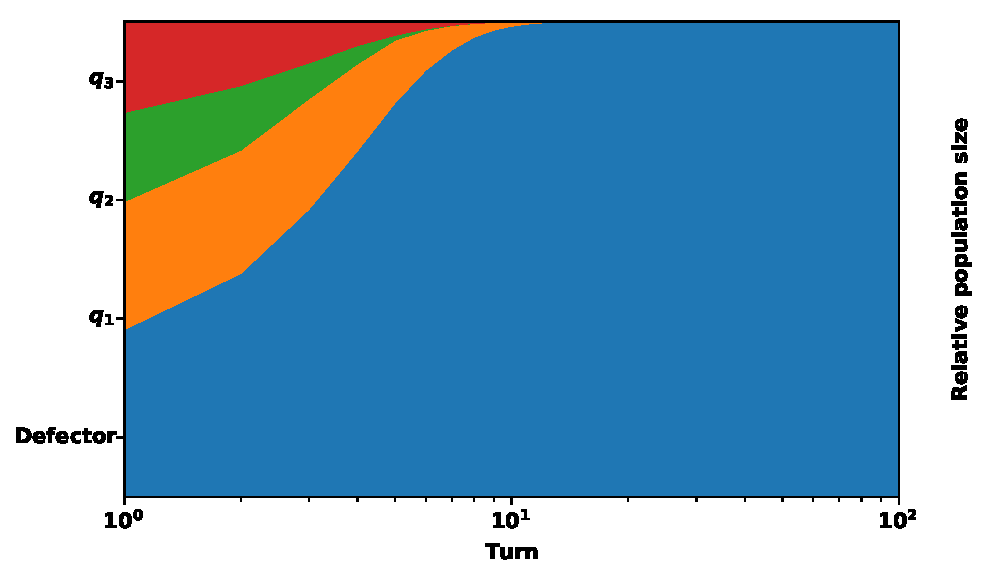
\includegraphics[width=\linewidth]{src/chapters/05/paper/Memory-size-in-the-prisoners-dilemma/img/population_defection_takes_over.pdf}
%         \caption{For opponents \(q_{1}=(\frac{371}{1250},\frac{4693}{25000},\frac{4037}{50000},\frac{18461}{25000})\),
%         $q_{2}=(\frac{48841}{100000},\frac{30587}{50000},\frac{76591}{100000},\frac{25921}{50000})$ and
%         $q_{3}=(\frac{22199}{100000},\frac{87073}{100000},\frac{646}{3125},\frac{91861}{100000})$
%         conditions (\ref{eq:defection_condition_one}) and
%         (\ref{eq:defection_condition_two}) hold and Defector takes over the
%         population.}
%         \label{fig:stable_defection}
%     \end{subfigure}\hfill
%     \begin{subfigure}{0.49\textwidth}
%         \centering
%         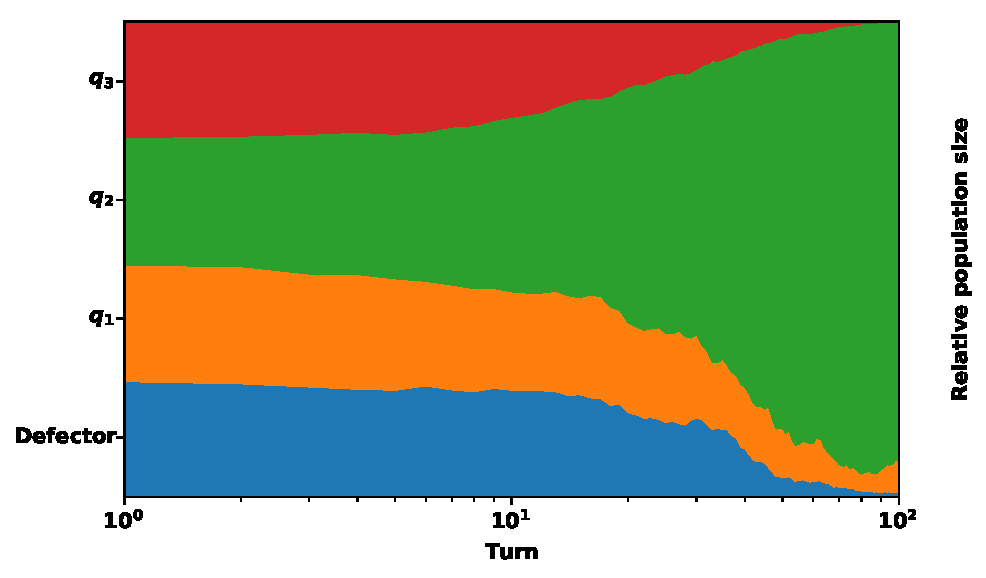
\includegraphics[width=\linewidth]{src/chapters/05/paper/Memory-size-in-the-prisoners-dilemma/img/population_defection_fails.pdf}
%         \caption{For opponents $q_{1}=(\frac{69773}{100000},\frac{21609}{100000},\frac{97627}{100000},\frac{623}{100000})$,
%         $q_{2}=(\frac{12649}{50000},\frac{43479}{100000},\frac{38969}{50000},\frac{19769}{100000})$ and
%         $q_{3}=(\frac{96703}{100000},\frac{54723}{100000},\frac{24317}{25000},\frac{35741}{50000})$
%         (\ref{eq:defection_condition_one}) fails and
%         (\ref{eq:defection_condition_two}) holds and Defector does not take over
%         the population.}
%         \label{fig:unstable_defection}
%     \end{subfigure}
% \end{figure}

% \section{Numerical experiments} \label{section:numerical_experiments}

% The results of this section rely on estimating best response memory-one strategies, but as stated in
% Section~\ref{section:best_response_mem_one}, estimating best responses
% analytically can quickly become an intractable problem. As a result, best
% responses will be estimated heuristically using Bayesian
% optimisation~\cite{Mokus1978}. Bayesian optimisation is a global optimisation
% algorithm that has proven to outperform many other popular
% algorithms~\cite{Jones2001}. The algorithm builds a bayesian understanding of
% the objective function which is well suited to the potential multiple local optimas in
% the described search space of this work. Differential evolution~\cite{Storn1997}
% was also considered, however, it was not selected due to Bayesian optimisation being
% computationally more efficient.

% As an example of the algorithm's usage let us consider the optimisation problem
% of (\ref{eq:mo_tournament_optimisation}). Figure~\ref{bayesian_example}
% illustrates the change of the utility function over iterations of the algorithm.
% The algorithm is set to run for 60 iterations. After 60 iterations if the
% utility has changed in the last 10\% iterations then algorithm runs for a
% further 20 iterations. This is repeated until there is no change to the utility
% in the last 10\% of iterations.


% \begin{figure}[!htbp]
%     \begin{center}
%     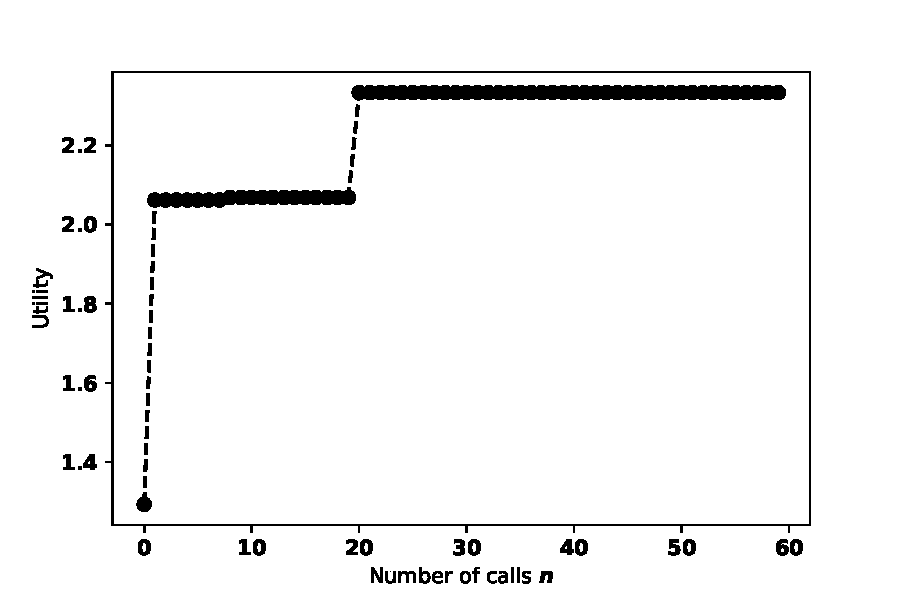
\includegraphics[width=.5\linewidth]{src/chapters/05/paper/Memory-size-in-the-prisoners-dilemma/img/bayesian_example.pdf}
%     \end{center}
%     \caption{Utility over time of calls using Bayesian optimisation. The
%     opponents are \(q^{(1)} = (\frac{1}{3}, \frac{1}{3}, \frac{1}{3},
%     \frac{1}{3})\) and \(q^{(2)} = (\frac{1}{3}, \frac{1}{3},
%     \frac{1}{3}, \frac{1}{3})\). The best response obtained is \(p^* = (0, \frac{11}{50}, 0, 0)\)}
%     \label{bayesian_example}
% \end{figure}

% The rest of the section is structured as follows. In
% Section~\ref{subsection:best_response_n_2}, Bayesian optimisation is used to
% generate a data set containing memory-one best responses against a number of
% random opponents. The extortionate behaviour of these best responses is then
% evaluated using a method introduced in~\cite{Knight2019}. In Section
% \ref{subsection:best_respnse_evolutionary_setting}, a similar data set and
% approach is discussed but this time the best responses are memory-one best
% responses in an evolutionary setting where they also incorporate self
% interactions. This has immediate applications to Moran processes.
% Finally, Section~\ref{subsection:longer_memory_best_response}
% compares the performances of memory-one and longer-memory best responses against
% a number of opponents.

% \subsection{Best response memory-one strategies for \(N=2\)}\label{subsection:best_response_n_2}

% As briefly discussed in Section~\ref{section:introduction}, zero-determinants
% have been praised for their robustness against a single opponent.
% Zero-determinants are evidence that extortion works in pairwise interactions,
% their behaviour ensures that the strategies will
% never lose a game. However, this paper
% argues that in multi opponent interactions, where the payoffs matter, strategies
% trying to exploit their opponents will suffer.

% Compared to zero-determinants, best response memory-one strategies which
% have a theory of mind of their opponents, utilise their behaviour in order to
% gain the most from their interactions. The question that arises then is whether
% best response strategies are optimal because they behave in an extortionate
% way. To estimate a strategy's extortionate
% behaviour the SSE method as described in~\cite{Knight2019} is used. SSE is
% defined as how far a strategy is from behaving extortionate, thus a high
% SSE implies a non extortionate behaviour.

% %TODO include explanation of SSE

% A data set of best response memory-one strategies with \(N=2\) opponents has been
% generated which is available at~\cite{glynatsi2019}. The data set contains a total of 1000 trials
% corresponding to 1000 different instances of a best response strategy. For each
% trial a set of 2 opponents is randomly generated and the memory-one best response
% against them is found. The probabilities \(q_i\) of the opponents are
% randomly generated and Figures~\ref{fig:first_opponents_probabilities} and
% \ref{fig:second_opponents_probabilities}, show that they are uniformly
% distributed over the trials. Thus, the full space of possible opponents has been
% covered.

% \begin{figure}[!htbp]
%     \begin{subfigure}{0.49\textwidth}
%         \centering
%         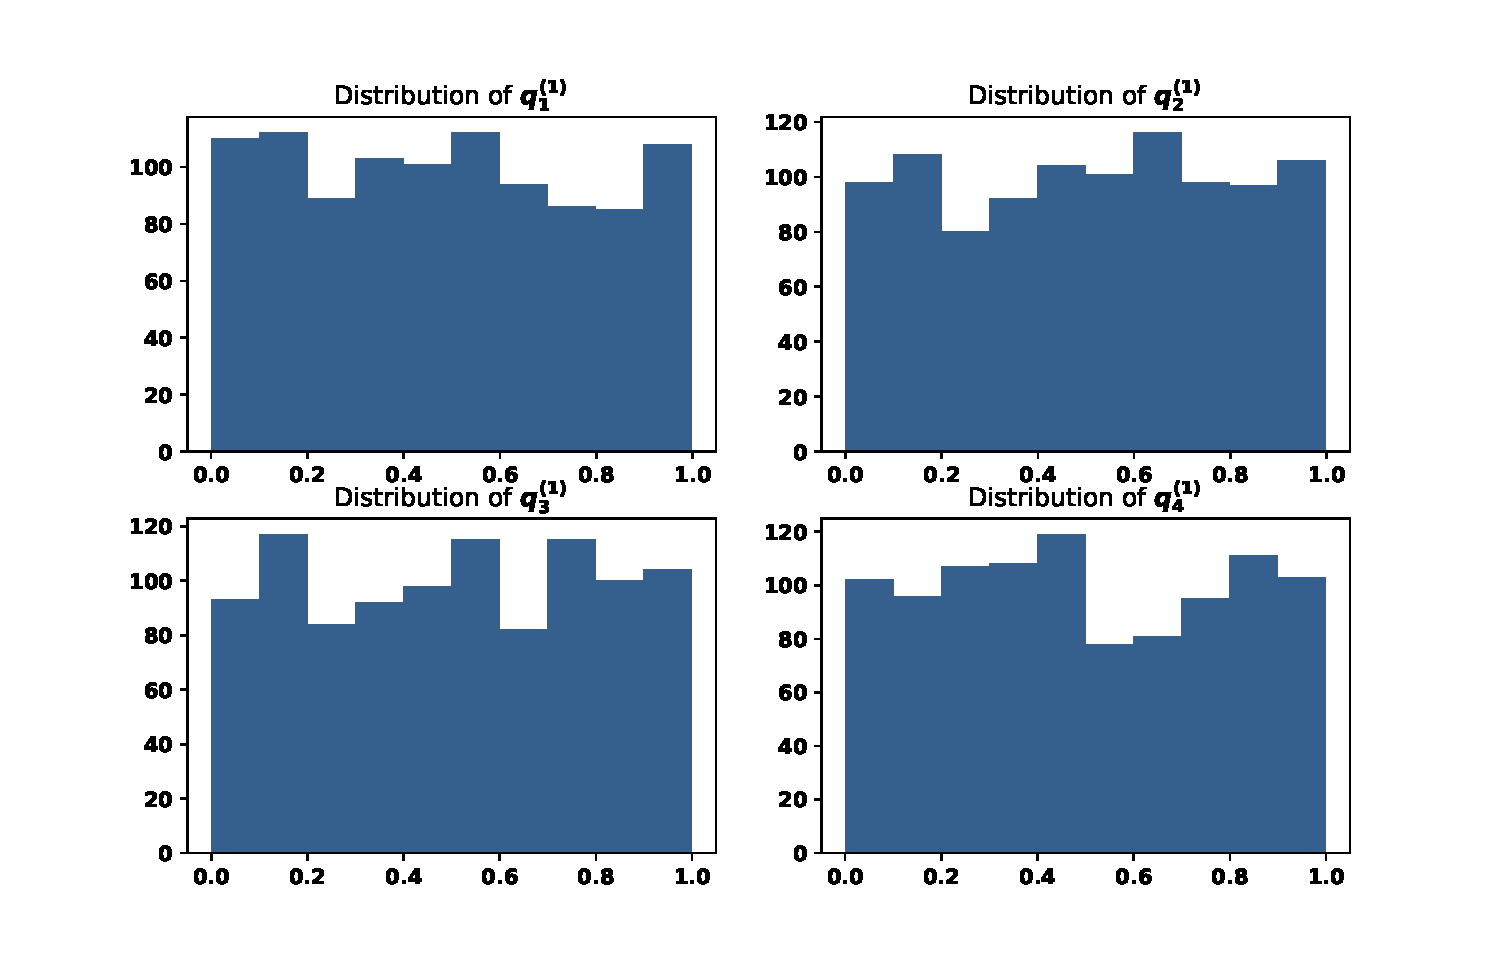
\includegraphics[width=\linewidth]{src/chapters/05/paper/Memory-size-in-the-prisoners-dilemma/img/first_opponent_probabilities.pdf}
%         \subcaption{Distributions of first opponents' probabilities.}
%         \label{fig:first_opponents_probabilities}
%     \end{subfigure}
%     \begin{subfigure}{0.49\textwidth}
%         \centering
%         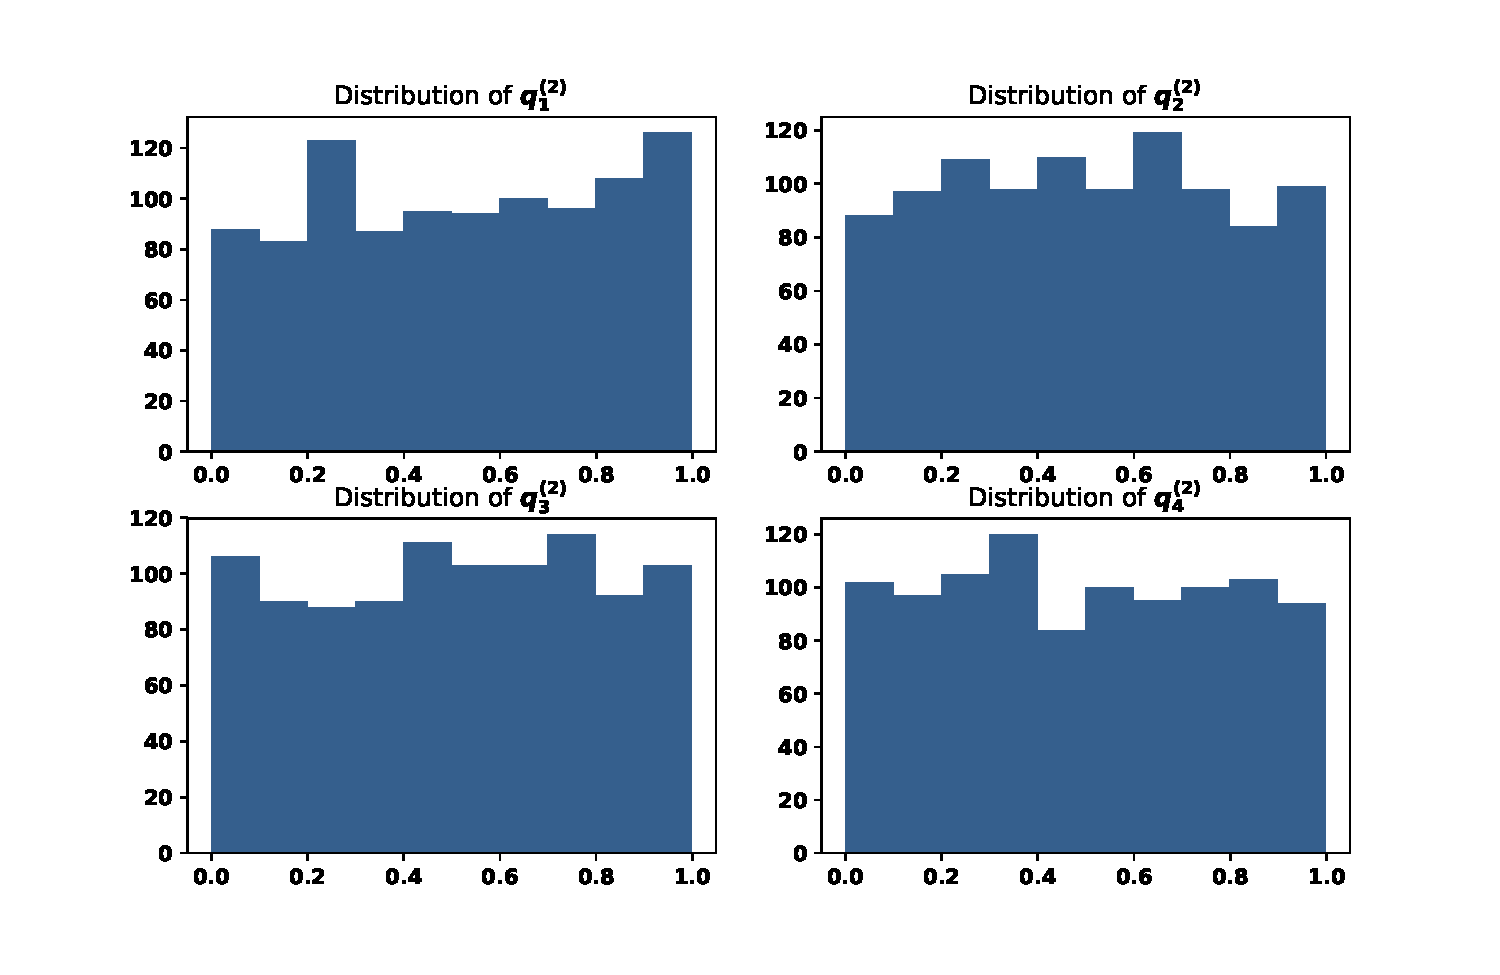
\includegraphics[width=\linewidth]{src/chapters/05/paper/Memory-size-in-the-prisoners-dilemma/img/second_opponent_probabilities.pdf}
%         \subcaption{Distributions of second opponents' probabilities.}
%         \label{fig:second_opponents_probabilities}
%     \end{subfigure}
% \end{figure}

% The SSE method has been applied to the data set. The distribution of SSE for the best response is given in
% Figure~\ref{fig:sserror_mem_one} and a statistics summary in
% Table~\ref{table:sserror_stats}. The distribution of SSE is skewed to the left,
% indicating that the best response does exhibit extortionate behaviour, however,
% the best response is not uniformly extortionate. A positive measure of skewness
% and kurtosis indicates a heavy tail to the right. Therefore, in several cases the
% strategy is not trying to extort its the opponents.

% So although the best response strategy can exhibit extortionate behaviour, its
% performance is maximised by behaving in a more adaptable way than zero-determinant
% strategies. This is confirms similar results such as~\cite{Knight2019}.
% This analysis will now be extended to an evolutionary setting.

% \begin{figure}[!htbp]
%     \begin{minipage}{0.72\textwidth}
%             \begin{center}
%                 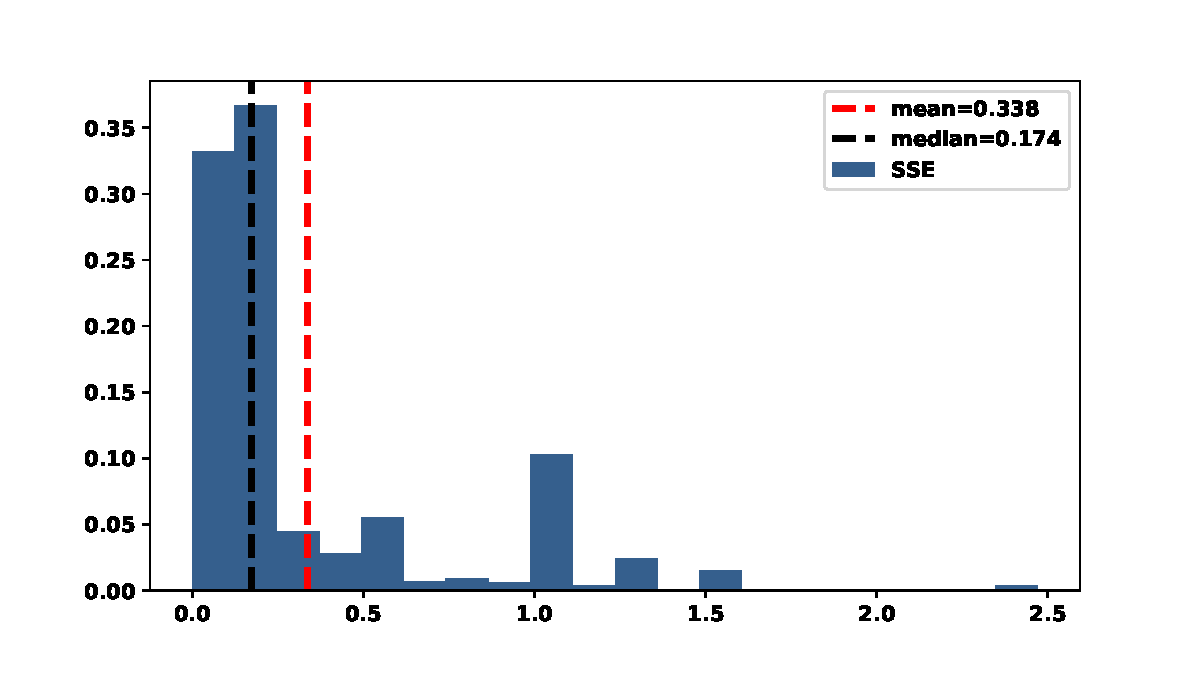
\includegraphics[width=\linewidth]{src/chapters/05/paper/Memory-size-in-the-prisoners-dilemma/img/best_respones_sserror.pdf}
%             \end{center}
%                 \caption{Distribution of SSE for memory-one best responses, when \(N=2\).}
%                 \label{fig:sserror_mem_one}
%     \end{minipage}\hspace{1cm}
%     \begin{minipage}{0.21\textwidth}
%         \centering
%         \captionsetup{type=table}
%         \resizebox{.85\columnwidth}{!}{%
%             \begin{tabular}{lr}
\toprule
{} &     SSE \\
\midrule
count  &  1000.00000 \\
mean   &     0.33762 \\
std    &     0.39667 \\
min    &     0.00000 \\
5\%     &     0.02078 \\
25\%    &     0.07597 \\
50\%    &     0.17407 \\
95\%    &     1.05943 \\
max    &     2.47059 \\
median &     0.17407 \\
skew   &     1.87231 \\
kurt   &     3.60029 \\
\bottomrule
\end{tabular}
}
%             \caption{Summary statistics SSE of best response memory one strategies included
%             tournaments of \(N=2\).}
%             \label{table:sserror_stats}
%       \end{minipage}
% \end{figure}

% \subsection{Memory-one best responses in evolutionary dynamics}\label{subsection:best_respnse_evolutionary_setting}

% As mentioned in Section~\ref{section:utility}, the IPD is commonly studied in
% Moran processes, and generally, in evolutionary processes. In these settings self
% interactions are key. This section extends the formulation of best responses
% in evolutionary dynamics, more specifically, the optimisation problem of
% (\ref{eq:mo_tournament_optimisation}) is extended to
% include self interactions.

% Self interactions can be incorporated in the formulation
% that has been used so far. The utility is given by,

% \begin{equation}
%     \frac{1}{N} \sum\limits_{i=1} ^ {N} {u_q}^{(i)} (p) + u_p(p)
% \end{equation}

% and the optimisation problem of (\ref{eq:mo_tournament_optimisation}) is modified to give:

% \begin{equation}\label{eq:mo_evolutionary_optimisation}
%     \begin{aligned}
%     \max_p: & \ \frac{1}{N} \sum\limits_{i=1} ^ {N} {u_q}^{(i)} (p) + u_p(p)
%     \\
%     \text{such that}: & \ p \in \R_{[0, 1]}
%     \end{aligned}
% \end{equation}

% % Note that exact formulate are known for given evolutionary processes, however,
% % for simplicity 17 is given to optimisation.
% For determining the memory-one best response in an evolutionary setting,
% an algorithmic approach is considered, called \textit{best
% response dynamics}. Best response dynamics are commonly used in evolutionary
% game theory. They represent a class of strategy updating rules, where players in
% the next round are determined by their best responses to some subset of the
% population. The best response dynamics approach used in this manuscript is given by
% Algorithm~\ref{algo:best_response_dynamics}.

% \begin{minipage}{.6\textwidth}
%     \begin{algorithm}[H]
%         $p^{(t)}\leftarrow (1, 1, 1, 1)$\;
%         \While{$p^{(t)} \neq p ^{(t -1)}$}{
%          $p^{(t + 1)} =  \text{argmax} \frac{1}{N} \sum\limits_{i=1} ^ {N} {u_q}^{(i)}
%          (p^{(t + 1)}) + u_p^{(t)}(p^{(t + 1)})$\;
%         }
%         \caption{Best response dynamics Algorithm}
%         \label{algo:best_response_dynamics}
%     \end{algorithm}
% \end{minipage}

% The best response dynamics algorithm starts by setting an initial
% solution \(p^{(1)}=(1, 1, 1, 1)\), and repeatedly finds a strategy that maximises
% (\ref{eq:mo_evolutionary_optimisation}) using Bayesian optimisation. The
% algorithm stops once a cycle (a sequence of iterated evaluated points) is
% detected. A numerical example of the algorithm is given in Figure~\ref{fig:best_response_dynamics_results}.

% \begin{figure}[!htbp]
%     \centering
%     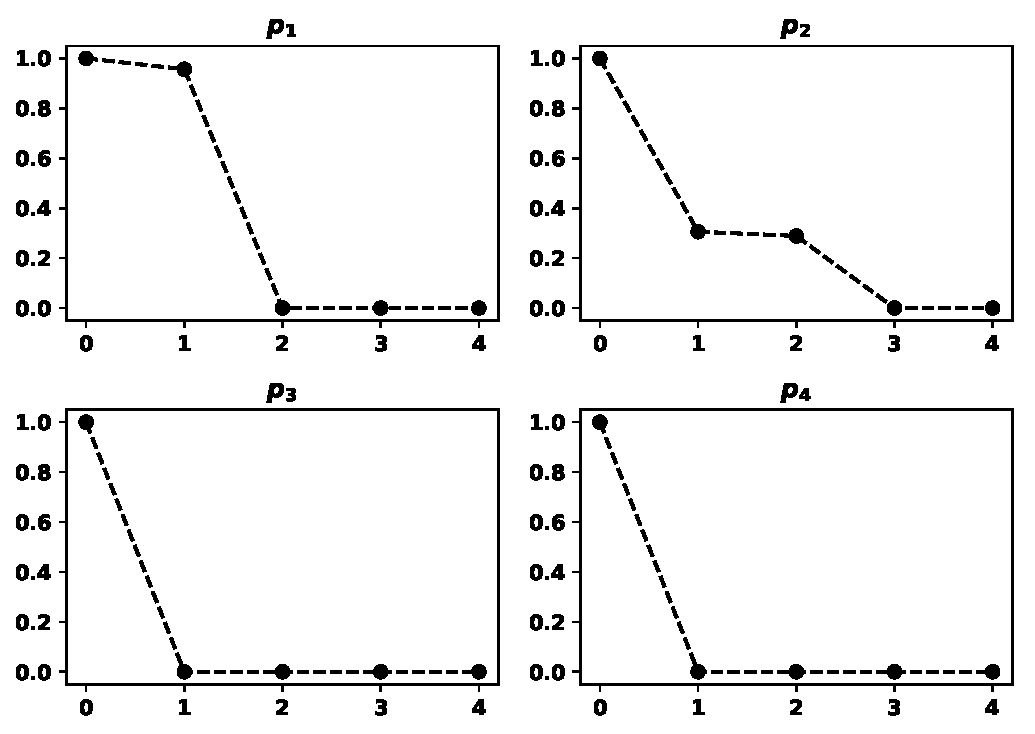
\includegraphics[width=.6\textwidth]{src/chapters/05/paper/Memory-size-in-the-prisoners-dilemma/img/evolution_example_two.pdf}
%     \caption{Best response dynamics with \(N=2\). More specifically, for
%     \(q ^{(1)}=(\frac{59}{250},
%                 \frac{1031}{10000},
%                 \frac{99}{250},
%                 \frac{1549}{10000})\) and
%     \(q ^{(2)}=(\frac{133}{2000},
%                 \frac{803}{2000},
%                 \frac{9179}{10000},
%                 \frac{2001}{2500})\).}
% \label{fig:best_response_dynamics_results}
% \end{figure}

% The algorithm has been used to estimate the best response in an evolutionary
% setting for each of the 1000 pairs of opponents described in
% Section~\ref{subsection:best_response_n_2}. These are also included in the data
% set~\cite{glynatsi2019}, and moreover, the SSE method has also been applied. The
% distribution of SSE is given by Figure~\ref{fig:sserror_mem_one} and a
% statistical summary by Table~\ref{table:sserror_stats}.

% Similarly to the results of Section~\ref{subsection:best_response_n_2}, the
% evolutionary best response strategy does not behave uniformly extortionately. A
% larger value of both the kurtosis and the skewness of the SSE distribution
% indicates that in evolutionary settings a memory-one best response is even more
% adaptable.

% The difference between best responses in tournaments and in evolutionary
% settings are further explored by Figure~\ref{fig:behaviour_violin_plots}.
% Though, Table~\ref{table:wilcoxon_tests} details that no statistically
% significant differences has been found, from
% Figure~\ref{fig:behaviour_violin_plots}, it seems that evolutionary best
% response has a higher $p_2$ median. Thus, they more likely to forgive after
% being tricked.

% \begin{figure}[!htbp]
%     \begin{minipage}{0.72\textwidth}
%             \begin{center}
%             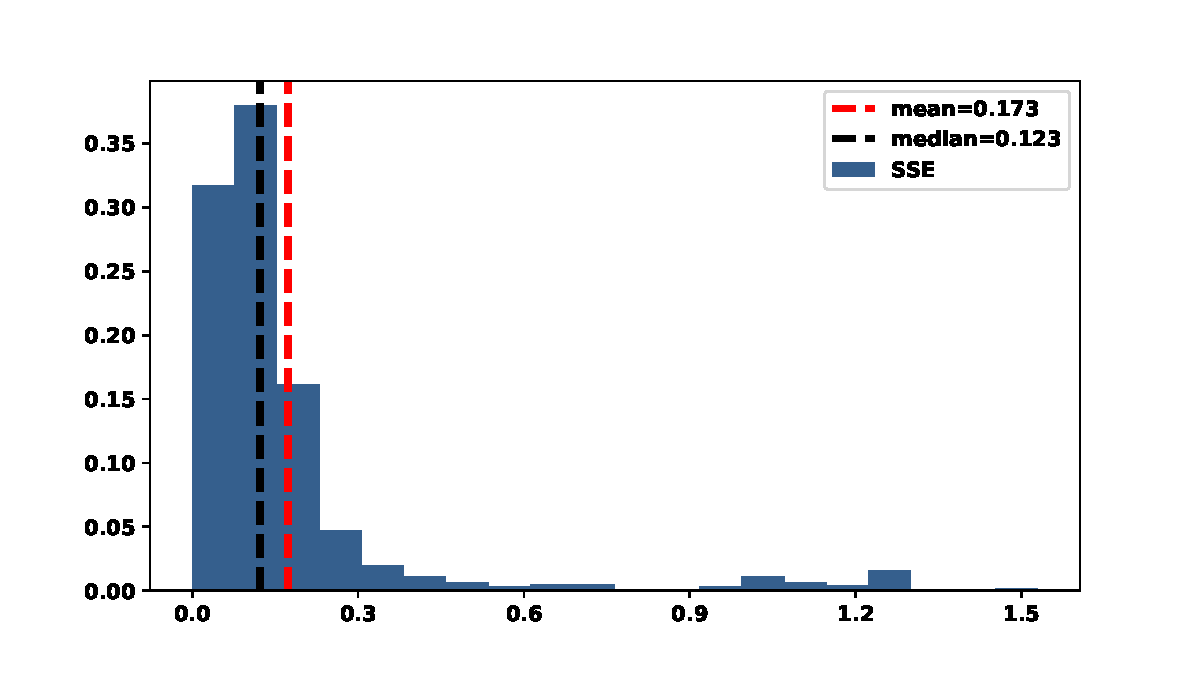
\includegraphics[width=\linewidth]{src/chapters/05/paper/Memory-size-in-the-prisoners-dilemma/img/evo_sserror.pdf}
%             \end{center}
%             \caption{Distribution of SSE of best response memory-one strategies in
%             evolutionary settings, when \(N=2\).}
%             \label{fig:sserror_mem_one}
%     \end{minipage}\hspace{1cm}
%     \begin{minipage}{0.21\textwidth}
%         \centering
%         \captionsetup{type=table}
%         \resizebox{.85\columnwidth}{!}{%
%             \begin{tabular}{lr}
\toprule
{} &  SSE \\
\midrule
count  &    1000.00000 \\
mean   &       0.17326 \\
std    &       0.23489 \\
min    &       0.00001 \\
5\%     &       0.01497 \\
25\%    &       0.05882 \\
50\%    &       0.12253 \\
95\%    &       0.67429 \\
max    &       1.52941 \\
median &       0.12253 \\
skew   &       3.41839 \\
kurt   &      11.92339 \\
\bottomrule
\end{tabular}
}
%             \caption{Summary statistics SSE of best response memory-one strategies in
%             evolutionary settings, when when \(N=2\).}
%             \label{table:sserror_stats}
%       \end{minipage}
% \end{figure}

% \begin{figure}[!htbp]
%     \centering
%     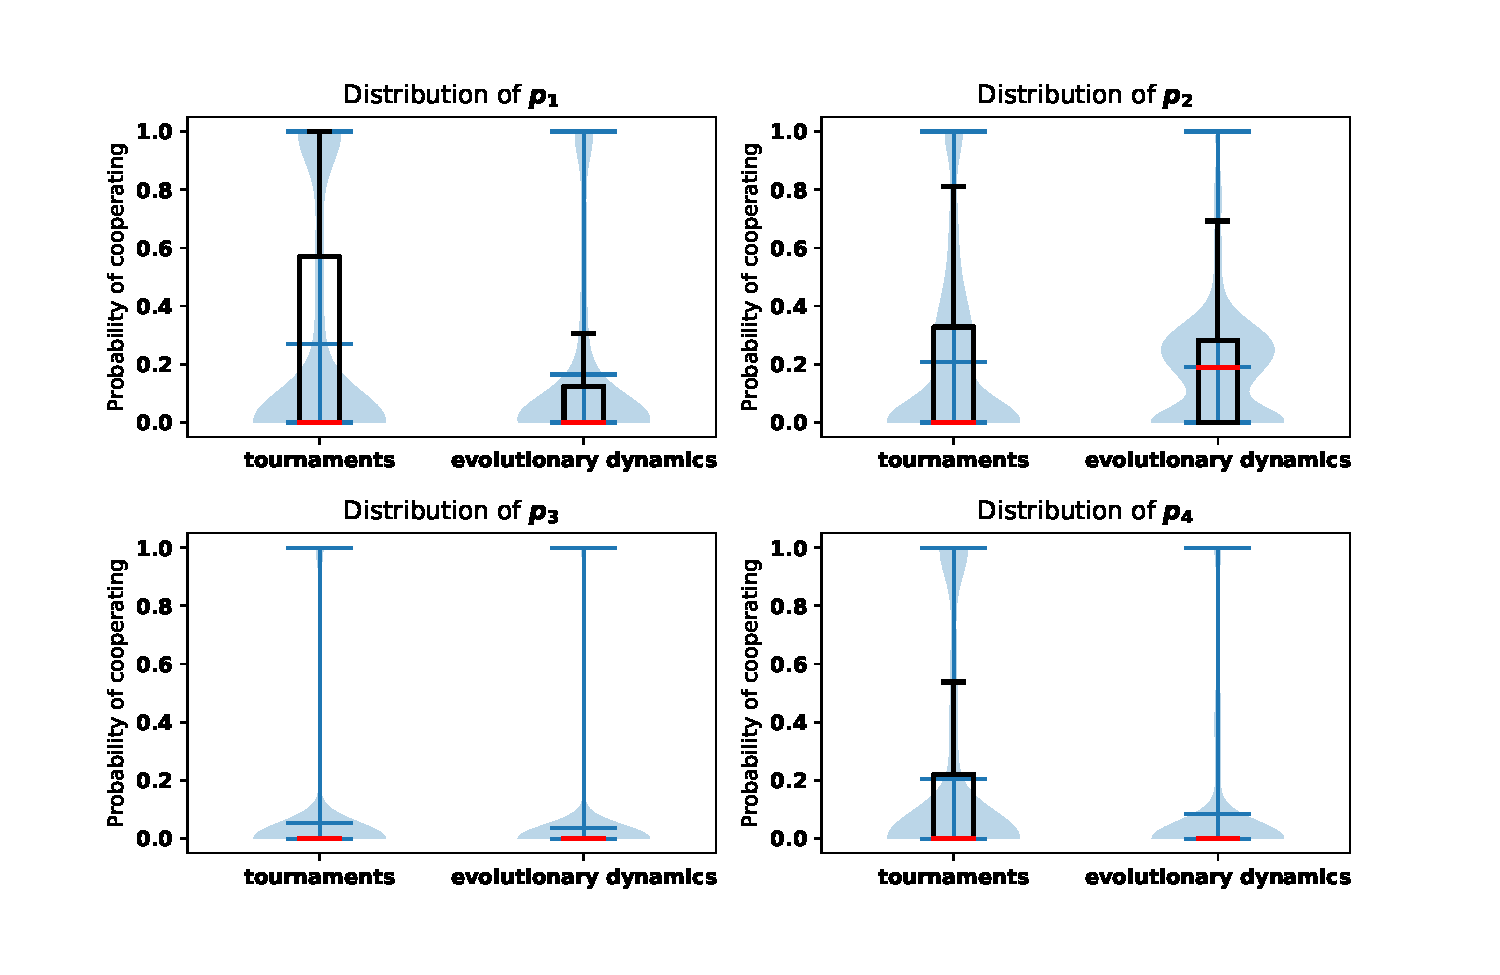
\includegraphics[width=.8\textwidth]{src/chapters/05/paper/Memory-size-in-the-prisoners-dilemma/img/behaviour_violin_plots.pdf}
%     \caption{Distributions of \(p^*\) for both best response and evolutionary memory-one
%     strategies.}
%     \label{fig:behaviour_violin_plots}
% \end{figure}

% \begin{table}[!htbp]
%     \centering
%     \resizebox{.7\columnwidth}{!}{%
%     \begin{tabular}{llrrr}
\toprule
{} & Best Response Median in: &  Tournament &  Evolutionary Settings &  p-values \\
\midrule
&       Distribution $p_1$ &         0.0 &                0.00000 &       0.0 \\
&       Distribution $p_2$ &         0.0 &                0.19847 &       0.0 \\
&       Distribution $p_3$ &         0.0 &                0.00000 &       0.0 \\
&       Distribution $p_4$ &         0.0 &                0.00000 &       0.0 \\
\bottomrule
\end{tabular}
}
%     \caption{A non parametric test, Wilcoxon Rank Sum, has been performed to
%     tests the difference in the median values of the cooperation probabilities
%     in tournaments versus evolutionary settings. A non parametric test is used because
%     is evident that the data are skewed.}\label{table:wilcoxon_tests}
% \end{table}

% \subsection{Longer memory best response}\label{subsection:longer_memory_best_response}

% This section focuses on the memory size of strategies. The effectiveness of
% memory in the IPD has been previously explored in the literature, as
% discussed in Section~\ref{section:introduction}, however, none of the
% previous works has compared the performance of longer-memory strategies to
% memory-one best responses.

% In~\cite{Harper2017}, a strategy called \textit{Gambler} which makes
% probabilistic decisions based on the opponent's \(n_1\) first moves, the
% opponent's \(m_1\) last moves and the player's \(m_2\) last moves was
% introduced. In this manuscript Gambler with parameters: $n_1 = 2, m_1 = 1$ and $m_2 = 1$ is used
% as a longer-memory strategy.

% By considering the opponent's first two moves, the opponents last move and the
% player's last move, there are only 16 $(4 \times 2 \times 2)$ possible outcomes
% that can occur, furthermore, Gambler also makes a probabilistic decision of
% cooperating in the opening move. Thus, Gambler is a function \(f: \{\text{C,
% D}\} \rightarrow [0, 1]_{\R}\). This can be hard coded as an element
% of \([0, 1]_{\R} ^ {16 + 1}\), one probability for each outcome plus the opening
% move. Hence, compared to (\ref{eq:mo_tournament_optimisation}), finding an
% optimal Gambler is a 17 dimensional problem given by:

% \begin{equation}\label{eq:gambler_optimisation}
%     \begin{aligned}
%     \max_p: & \ \sum_{i=1} ^ {N} {U_q}^{(i)} (f)
%     \\
%     \text{such that}: & \ f \in \R_{[0, 1]}^{17}
%     \end{aligned}
% \end{equation}

% Note that (\ref{eq:tournament_utility}) can not be used here for the utility
% of Gambler, and actual simulated players are used. This is done using~\cite{axelrodproject}
% with 500 turns and 200 repetitions, moreover, (\ref{eq:gambler_optimisation})
% is solved numerically using Bayesian optimisation.

% Similarly to previous sections, a large data set has been generated with
% instances of an optimal Gambler and a memory-one best response, available
% at~\cite{glynatsi2019}. Estimating a best response Gambler (17 dimensions) is
% computational more expensive compared to a best response memory-one (4
% dimensions). As a result, the analysis of this section is based on a total of
% 130 trials. For each trial two random opponents have been selected. The 130 pair
% of opponents are a sub set of the opponents used in
% Section~\ref{subsection:best_response_n_2}-
% \ref{subsection:best_respnse_evolutionary_setting}. The distributions of their
% transition probabilities are given in Figures
% \ref{fig:first_opponents_probabilities_with_gambler} and
% \ref{fig:first_opponents_probabilities_with_gambler}.

% \begin{figure}[!htbp]
%     \begin{subfigure}{0.49\textwidth}
%         \centering
%         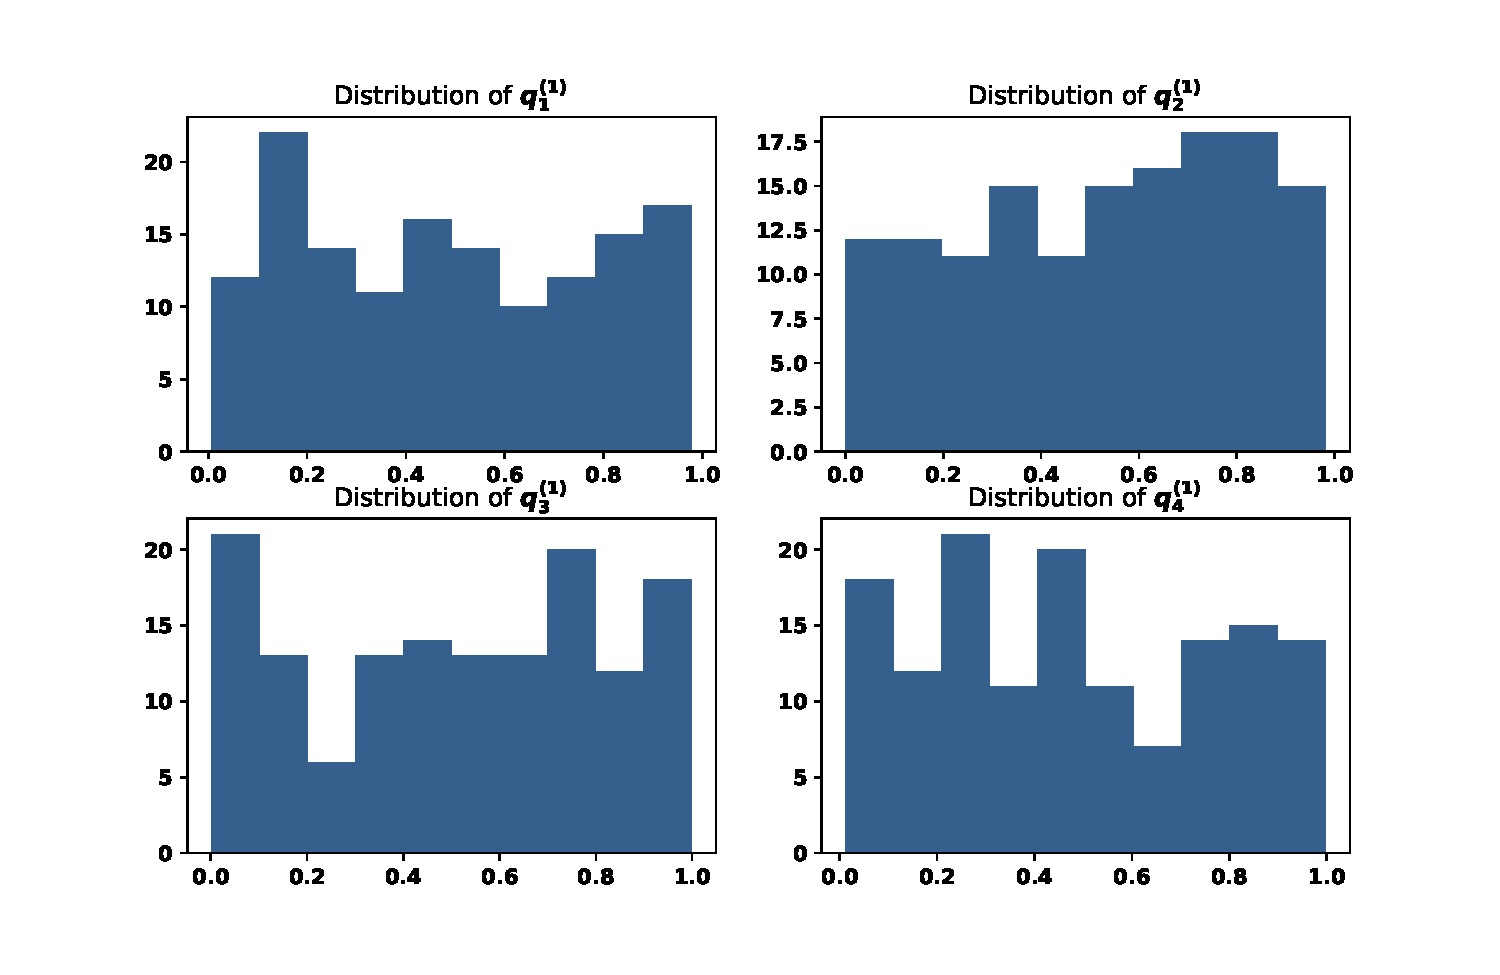
\includegraphics[width=\linewidth]{src/chapters/05/paper/Memory-size-in-the-prisoners-dilemma/img/first_opponent_probabilities_with_gambler.pdf}
%         \subcaption{Distributions of first opponents' probabilities for longer memory experiment.}
%         \label{fig:first_opponents_probabilities_with_gambler}
%     \end{subfigure}
%     \begin{subfigure}{0.49\textwidth}
%         \centering
%         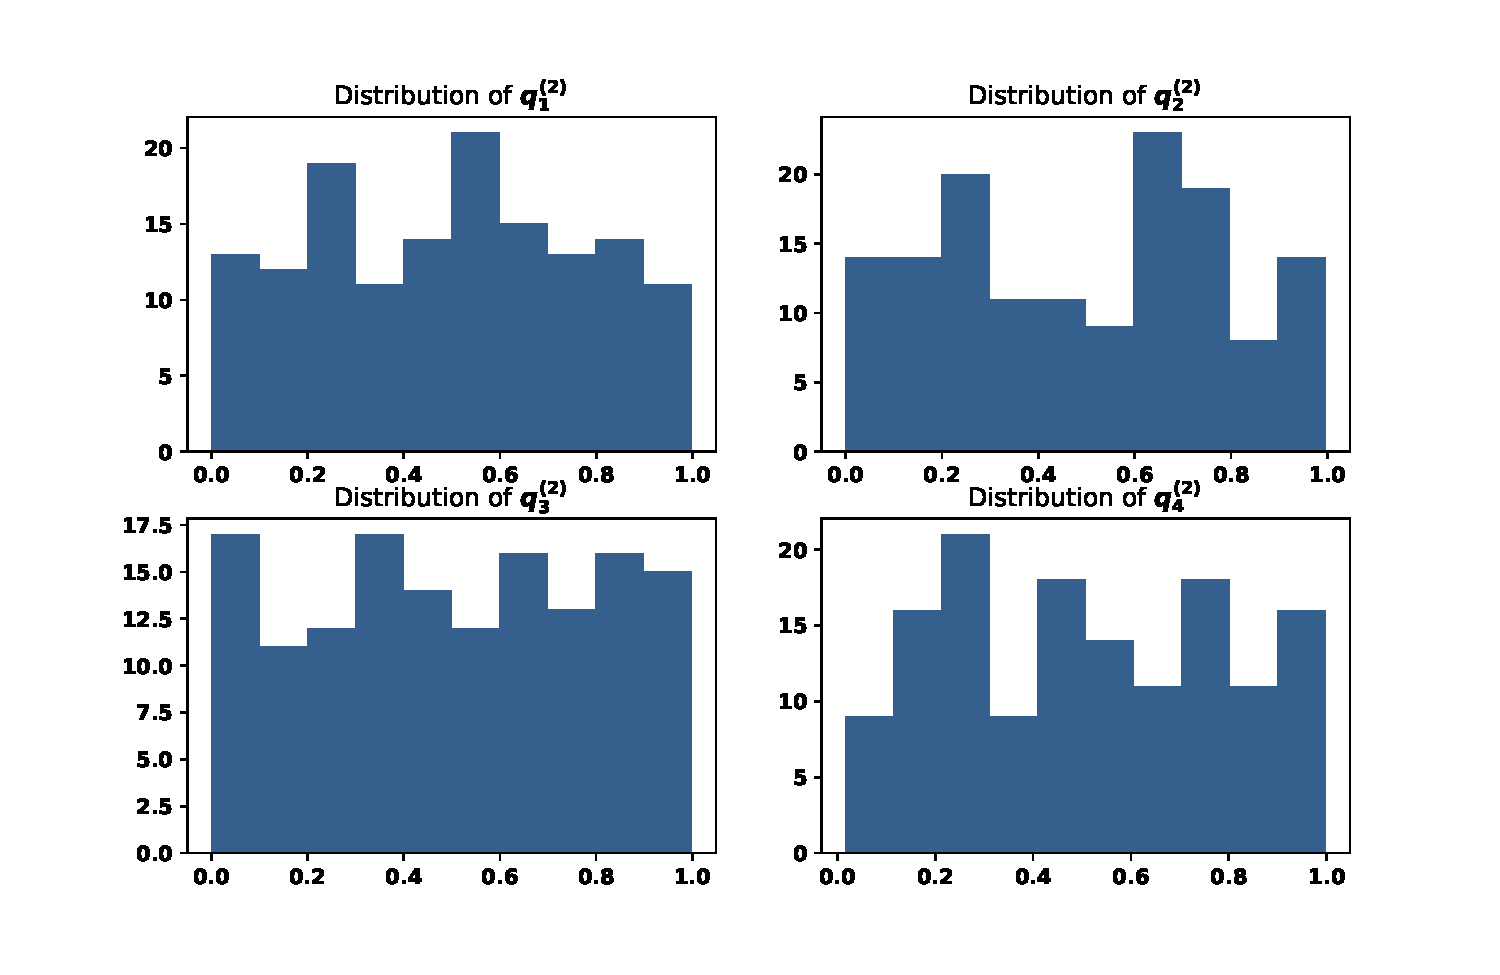
\includegraphics[width=\linewidth]{src/chapters/05/paper/Memory-size-in-the-prisoners-dilemma/img/second_opponent_probabilities_with_gambler.pdf}
%         \subcaption{Distributions of second opponents' probabilities for longer memory experiment.}
%         \label{fig:second_opponents_probabilities_with_gambler}
%     \end{subfigure}
% \end{figure}

% The utilities of both strategies are plotted against each other in
% Figure~\ref{fig:utilities_gambler_mem_one}. Although Gambler has an infinite
% memory (in order to remember the opening moves of the opponent) the information
% the strategy considers is not significantly larger than memory-one strategies.
% Even so, it is evident from Figure~\ref{fig:utilities_gambler_mem_one} that
% Gambler always performs as well as the best response memory-one or better. This seems to be at odd with the
% result of~\cite{Press2012} that against a memory-one opponent having a longer memory
% will not give a strategy any
% advantage. However, against two memory-one opponents Gambler's performance is better than
% the optimal memory-one strategy. This is evidence that in the case of two opponents having a
% shorter memory is limiting.

% \begin{figure}[!htbp]
%     \centering
%     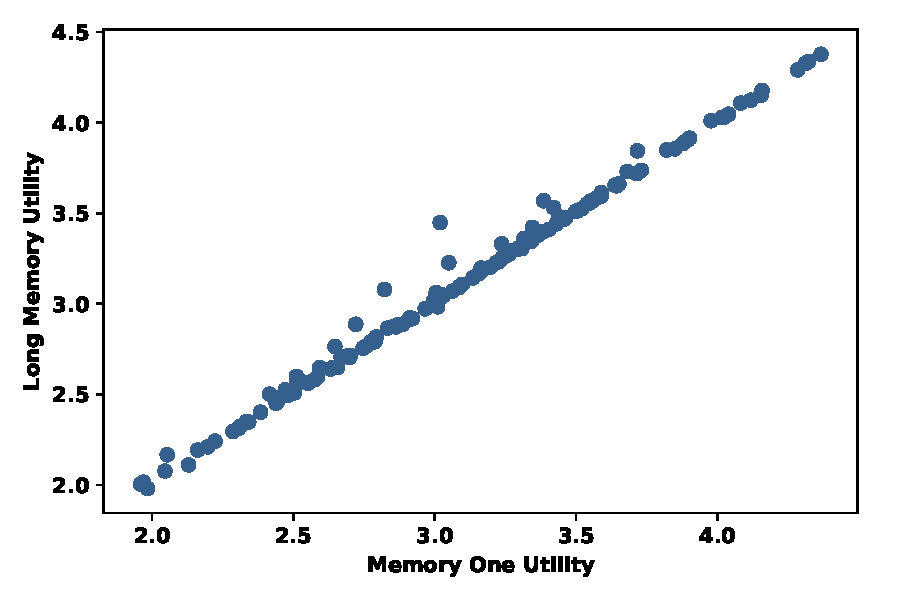
\includegraphics[width=.55\textwidth]{src/chapters/05/paper/Memory-size-in-the-prisoners-dilemma/img/gambler_performance_against_mem_one.pdf}
%     \caption{Utilities of Gambler and best response memory-one strategies for
%     130 different pair of opponents.}\label{fig:utilities_gambler_mem_one}
% \end{figure}

% \section{Conclusion}

% This manuscript has considered \textit{best response} strategies in the IPD game, and
% more specifically, \textit{memory-one best responses}. It has proven that there is
% a compact way of identifying a memory-one best response to a group of opponents,
% and moreover, that there exists a condition for which in an
% environment of memory-one opponents defection is the stable choice.
% The later parts of this paper focused on a series of empirical results, where it
% was shown that the performance and the evolutionary stability of memory-one
% strategies rely not on extortion but on adaptability. Finally, it was shown that
% memory-one strategies' performance is limited by their memory in cases where
% they interact with multiple opponents.

% Following the work described in~\cite{Nowak1989}, where it was shown that the
% utility between two memory-one strategies can be estimated by a Markov
% stationary state, we proved that the utilities can be written as a ration of two
% quadratic forms in $R^4$, Theorem~\ref{theorem:quadratic_form_u}. This was
% extended to include multiple opponents, as the IPD is commonly studied in such
% situations, Theorem~\ref{theorem:tournament_utility}.
% The formulation of Theorem~\ref{theorem:tournament_utility} allowed us to introduce an approach for identifying
% memory-one best responses to any number of opponents;
% Lemma~\ref{lemma:memone_group_best_response}. This does not only have game
% theoretic novelty, but also a mathematical novelty of solving quadratic ratio
% optimisation problem where the quadratics are non concave. The results of
% Lemma~\ref{lemma:memone_group_best_response} were also used to define a
% condition for which defection is known to be stable.

% This manuscript presented several experimental results. These results were mainly to
% investigate the behaviour of memory-one strategies and their limitations. In
% Sections~\ref{subsection:best_response_n_2}
% and~\ref{subsection:best_respnse_evolutionary_setting}, a large data set which
% contained best responses in tournaments and in evolutionary settings for $N=2$
% was generated. This allowed us to investigate their respective behaviours, and
% whether it was extortionate acts that made them the most favourable strategies.
% However, it was shown that it was not extortion but adaptability that allowed
% the strategies to gain the most from their interactions.
% In evolutionary settings it was specifically shown that being adaptable and being
% able to forgive after being tricked were key factors. In Section~\ref{subsection:longer_memory_best_response}, the performance of
% memory-one strategies was put against the performance of a longer memory
% strategy called Gambler. There were several cases where Gambler would outperform
% the memory-one strategy, however, a memory-one strategy never managed to outperform
% a Gambler. This result occurred whilst considering a Gambler with a sufficiently
% larger memory but not a sufficiently larger amount of information regarding
% the game.

% All the empirical results presented in this manuscript have been for the
% case of $N=2$. In future work we would consider larger values of $N$, however, we
% believe that for larger values of $N$ the results that have been presented here would
% only be more evident.

% \section{Acknowledgements}

% A variety of software libraries have been used in this work:

% \begin{itemize}
%     \item The Axelrod library for IPD simulations~\cite{axelrodproject}.
%     \item The Scikit-optimize library for an implementation of Bayesian optimisation~\cite{tim_head_2018_1207017}.
%     \item The Matplotlib library for visualisation~\cite{hunter2007matplotlib}.
%     \item The SymPy library for symbolic mathematics~\cite{sympy}.
%     \item The Numpy library for data manipulation~\cite{walt2011numpy}.
% \end{itemize}

% % Bibliography
% \bibliographystyle{plain}
% \bibliography{bibliography.bib}


% \section{Proofs of the Theorems}\label{section:appendix_a}

% \subsection{Proof of Theorem~\ref{theorem:quadratic_form_u}}\label{appendix:proof_theorem_one}
% The utility of a memory one player \(p\) against an opponent \(q\),
\(u_q(p)\), can be written as a ratio of two quadratic forms on \(R^4\).

\begin{proof}

In Section~\ref{section:utility}, it was discussed that \(u_q(p)\) it's the product
of the steady states \(v\) and the PD payoffs,

\[u_q(p) = v \cdot (R, S, T, P).\]

More specifically, with \((R, P, S, T) = (3, 1, 0, 5)\)

\begingroup
\footnotesize
\begin{equation}
    u_q(p) =
    \left(
      \frac
        {\parbox{6in}{$
            p_{1} p_{2} (q_{1} q_{2} - 5 q_{1} q_{4} - q_{1} - q_{2} q_{3} + 5 q_{3} q_{4} + q_{3}) + p_{1} p_{3} (- q_{1} q_{3} + q_{2} q_{3}) + p_{1} p_{4} (5 q_{1} q_{3} - 5 q_{3} q_{4}) + p_{3} p_{4} (- 3 q_{2} q_{3} + 3 q_{3} q_{4}) +$ \\
            \hspace*{1cm} $ p_{2} p_{3} (- q_{1} q_{2} + q_{1} q_{3} + 3 q_{2} q_{4} + q_{2} - 3 q_{3} q_{4} - q_{3}) + p_{2} p_{4} (- 5 q_{1} q_{3} + 5 q_{1} q_{4} + 3 q_{2} q_{3} - 3 q_{2} q_{4} + 2 q_{3} - 2 q_{4}) + $ \\
            \hspace*{1cm} $ p_{1} (- q_{1} q_{2} + 5 q_{1} q_{4} + q_{1}) + p_{2} (q_{2} q_{3} - q_{2} - 5 q_{3} q_{4} - q_{3} + 5 q_{4} + 1) + p_{3} (q_{1} q_{2} - q_{2} q_{3} - 3 q_{2} q_{4} - q_{2} + q_{3}) +$ \\
            \hspace*{4cm} $ p_{4} (- 5 q_{1} q_{4} + 3 q_{2} q_{4} + 5 q_{3} q_{4} - 5 q_{3} + 2 q_{4}) + q_{2} - 5 q_{4} - 1$
        }}
        {\parbox{6in}{$
        p_{1} p_{2} (q_{1} q_{2} - q_{1} q_{4} - q_{1} - q_{2} q_{3} + q_{3} q_{4} + q_{3}) + p_{1} p_{3} (- q_{1} q_{3} + q_{1} q_{4} + q_{2} q_{3} - q_{2} q_{4}) + p_{1} p_{4} (- q_{1} q_{2} + q_{1} q_{3} + q_{1} + q_{2} q_{4} - q_{3} q_{4} - q_{4}) +$ \\
        $ p_{2} p_{3} (- q_{1} q_{2} + q_{1} q_{3} + q_{2} q_{4} + q_{2} - q_{3} q_{4} - q_{3}) + p_{2} p_{4} (- q_{1} q_{3} + q_{1} q_{4} + q_{2} q_{3} - q_{2} q_{4}) + p_{3} p_{4} (q_{1} q_{2} - q_{1} q_{4} - q_{2} q_{3} - q_{2} + q_{3} q_{4} + q_{4}) + $ \\
        $ p_{1} (- q_{1} q_{2} + q_{1} q_{4} + q_{1}) + p_{2} (q_{2} q_{3} - q_{2} - q_{3} q_{4} - q_{3} + q_{4} + 1) + p_{3} (q_{1} q_{2} - q_{2} q_{3} - q_{2} + q_{3} - q_{4}) + p_{4} (- q_{1} q_{4} + q_{2} + q_{3} q_{4} - q_{3} + q_{4} - 1) + $ \\
        \hspace*{7cm} $q_{2} - q_{4} - 1$
      }}
    \right).
\end{equation}
\endgroup

Let us consider the numerator of the \(u_q(p)\). The cross product terms \(p_ip_j\)
are given by,

\begingroup
\footnotesize
\begin{align*}
p_{1} p_{2} (q_{1} q_{2} - 5 q_{1} q_{4} - q_{1} - q_{2} q_{3} + 5 q_{3} q_{4}
+ q_{3}) + p_{1} p_{3} (- q_{1} q_{3} + q_{2} q_{3}) + p_{1} p_{4} (5 q_{1} q_{3} -
5 q_{3} q_{4}) + p_{3} p_{4} (- 3 q_{2} q_{3} + 3 q_{3} q_{4}) +  \\
p_{2} p_{3} (- q_{1} q_{2} + q_{1} q_{3} + 3 q_{2} q_{4} + q_{2} - 3 q_{3} q_{4} - q_{3}) +
p_{2} p_{4} (- 5 q_{1} q_{3} + 5 q_{1} q_{4} + 3 q_{2} q_{3} - 3 q_{2} q_{4} +
2 q_{3} - 2 q_{4}).
\end{align*}
\endgroup

This can be re written in a matrix format given by (\ref{eq:cross_product_coeffs}).

\begin{equation}\label{eq:cross_product_coeffs}
    \resizebox{0.8\linewidth}{!}{\arraycolsep=2.5pt%
    \boldmath\( 
    (p_1, p_2, p_3, p_4) \frac{1}{2} \left[\begin{matrix}0 & - \left(q_{1} - q_{3}\right) \left(q_{2} - 5 q_{4} - 1\right) & q_{3} \left(q_{1} - q_{2}\right) & - 5 q_{3} \left(q_{1} - q_{4}\right)\\- \left(q_{1} - q_{3}\right) \left(q_{2} - 5 q_{4} - 1\right) & 0 & \left(q_{2} - q_{3}\right) \left(q_{1} - 3 q_{4} - 1\right) & \left(q_{3} - q_{4}\right) \left(5 q_{1} - 3 q_{2} - 2\right)\\q_{3} \left(q_{1} - q_{2}\right) & \left(q_{2} - q_{3}\right) \left(q_{1} - 3 q_{4} - 1\right) & 0 & 3 q_{3} \left(q_{2} - q_{4}\right)\\- 5 q_{3} \left(q_{1} - q_{4}\right) & \left(q_{3} - q_{4}\right) \left(5 q_{1} - 3 q_{2} - 2\right) & 3 q_{3} \left(q_{2} - q_{4}\right) & 0\end{matrix}\right] \begin{pmatrix} 
    p_1 \\
    p_2 \\
    p_3 \\
    p_4 \end{pmatrix}
    \) }
\end{equation}

Similarly, the linear terms are given by,

\begingroup
\footnotesize
\begin{align*}
p_{1} (- q_{1} q_{2} + 5 q_{1} q_{4} + q_{1}) + p_{2} (q_{2} q_{3} - q_{2} - 5 q_{3} q_{4} - q_{3} + 5 q_{4} + 1) + p_{3} (q_{1} q_{2} - q_{2} q_{3} - 3 q_{2} q_{4} - q_{2} + q_{3}) + \\
p_{4} (- 5 q_{1} q_{4} + 3 q_{2} q_{4} + 5 q_{3} q_{4} - 5 q_{3} + 2 q_{4}).
\end{align*}
\endgroup

and the expression can be written using a matrix format as (\ref{eq:linear_coeffs}).

\begin{equation}\label{eq:linear_coeffs}
    \resizebox{0.38\linewidth}{!}{\arraycolsep=2.5pt%
    \boldmath\(
    (p_1, p_2, p_3, p_4) \left[\begin{matrix}q_{1} \left(q_{2} - 5 q_{4} - 1\right)\\- \left(q_{3} - 1\right) \left(q_{2} - 5 q_{4} - 1\right)\\- q_{1} q_{2} + q_{2} q_{3} + 3 q_{2} q_{4} + q_{2} - q_{3}\\5 q_{1} q_{4} - 3 q_{2} q_{4} - 5 q_{3} q_{4} + 5 q_{3} - 2 q_{4}\end{matrix}\right]\)}
\end{equation}

Finally, the constant term of the numerator, which is obtained by substituting
$p=(0, 0, 0, 0)$, is given by (\ref{eq:constant}).

\begin{equation}\label{eq:constant}
q_{2} - 5 q_{4} - 1
\end{equation}

Combining equations (\ref{eq:cross_product_coeffs}), (\ref{eq:linear_coeffs}) and (\ref{eq:constant})
gives that the numerator of \(u_q(p)\) can be written as,

\begingroup
\tiny\boldmath
\begin{align*}
    \frac{1}{2}p & \left[\begin{matrix}0 & - \left(q_{1} - q_{3}\right) \left(q_{2} - 5 q_{4} - 1\right) & q_{3} \left(q_{1} - q_{2}\right) & - 5 q_{3} \left(q_{1} - q_{4}\right)\\- \left(q_{1} - q_{3}\right) \left(q_{2} - 5 q_{4} - 1\right) & 0 & \left(q_{2} - q_{3}\right) \left(q_{1} - 3 q_{4} - 1\right) & \left(q_{3} - q_{4}\right) \left(5 q_{1} - 3 q_{2} - 2\right)\\q_{3} \left(q_{1} - q_{2}\right) & \left(q_{2} - q_{3}\right) \left(q_{1} - 3 q_{4} - 1\right) & 0 & 3 q_{3} \left(q_{2} - q_{4}\right)\\- 5 q_{3} \left(q_{1} - q_{4}\right) & \left(q_{3} - q_{4}\right) \left(5 q_{1} - 3 q_{2} - 2\right) & 3 q_{3} \left(q_{2} - q_{4}\right) & 0\end{matrix}\right] p^T +  \\
    & \left[\begin{matrix}0 & - \left(q_{1} - q_{3}\right) \left(q_{2} - 5 q_{4} - 1\right) & q_{3} \left(q_{1} - q_{2}\right) & - 5 q_{3} \left(q_{1} - q_{4}\right)\\- \left(q_{1} - q_{3}\right) \left(q_{2} - 5 q_{4} - 1\right) & 0 & \left(q_{2} - q_{3}\right) \left(q_{1} - 3 q_{4} - 1\right) & \left(q_{3} - q_{4}\right) \left(5 q_{1} - 3 q_{2} - 2\right)\\q_{3} \left(q_{1} - q_{2}\right) & \left(q_{2} - q_{3}\right) \left(q_{1} - 3 q_{4} - 1\right) & 0 & 3 q_{3} \left(q_{2} - q_{4}\right)\\- 5 q_{3} \left(q_{1} - q_{4}\right) & \left(q_{3} - q_{4}\right) \left(5 q_{1} - 3 q_{2} - 2\right) & 3 q_{3} \left(q_{2} - q_{4}\right) & 0\end{matrix}\right] p + q_{2} - 5 q_{4} - 1
\end{align*}
\endgroup

and equivalently as,

\[\frac{1}{2}pQp^T + cp + a\]

where \(Q\) \(\in \R^{4\times4}\) is a square matrix defined by the
transition probabilities of the opponent \(q_1, q_2, q_3, q_4\) as follows:

\begin{equation*}
    \resizebox{0.9\linewidth}{!}{\arraycolsep=2.5pt%
    \boldmath\(
    Q = \left[\begin{matrix}0 & - \left(q_{1} - q_{3}\right) \left(q_{2} - 5 q_{4} - 1\right) & q_{3} \left(q_{1} - q_{2}\right) & - 5 q_{3} \left(q_{1} - q_{4}\right)\\- \left(q_{1} - q_{3}\right) \left(q_{2} - 5 q_{4} - 1\right) & 0 & \left(q_{2} - q_{3}\right) \left(q_{1} - 3 q_{4} - 1\right) & \left(q_{3} - q_{4}\right) \left(5 q_{1} - 3 q_{2} - 2\right)\\q_{3} \left(q_{1} - q_{2}\right) & \left(q_{2} - q_{3}\right) \left(q_{1} - 3 q_{4} - 1\right) & 0 & 3 q_{3} \left(q_{2} - q_{4}\right)\\- 5 q_{3} \left(q_{1} - q_{4}\right) & \left(q_{3} - q_{4}\right) \left(5 q_{1} - 3 q_{2} - 2\right) & 3 q_{3} \left(q_{2} - q_{4}\right) & 0\end{matrix}\right]\)},
\end{equation*}

\(c\) \(\in \R^{4 \times 1}\) is similarly defined by:

\begin{equation*}
    \resizebox{0.3\linewidth}{!}{\arraycolsep=2.5pt%
    \boldmath\(c = \left[\begin{matrix}q_{1} \left(q_{2} - 5 q_{4} - 1\right)\\- \left(q_{3} - 1\right) \left(q_{2} - 5 q_{4} - 1\right)\\- q_{1} q_{2} + q_{2} q_{3} + 3 q_{2} q_{4} + q_{2} - q_{3}\\5 q_{1} q_{4} - 3 q_{2} q_{4} - 5 q_{3} q_{4} + 5 q_{3} - 2 q_{4}\end{matrix}\right]\),}
\end{equation*}

and \(a = - q_{2} + 5 q_{4} + 1\).

The same process is done for the denominator.
\end{proof}

% \subsection{Proof of Theorem~\ref{theorem:concavity}}\label{appendix:proof_theorem_three}
% The utility \(u_q(p)\) is non concave and neither are it's numerator or
denominator. Furthermore, the denominator is not always strictly positive.

\begin{proof}

The utility \(u_q(p)\) is non concave because the concavity condition fails for at
least one pair of points see Appendix~\ref{appendix:non_concave}.

Furthermore, regarding the numerator and denominator of \(u_q(p)\)
in~\cite{Anton2014} it is stated that a quadratic form will be concave if and
only if it's symmetric matrix is semi-negative definite. A matrix \(A\) is
semi-negative definite if:

\begin{equation}\label{def:semi_negative}
|A|_i \leq 0 \text{ for } i \text{ is odd and } |A|_i \geq 0  \text{ for } i
\text{ is even,}
\end{equation}

where \(|A|_i\) is the eigenvalues of the submatrix \(A_i\).

For (\ref{eq:optimisation_quadratic}), neither \(\frac{1}{2}pQp^T + cp + a\)
or \(\frac{1}{2}p\bar{Q}p^T + \bar{c}p + \bar{a}\) are concave because for an even \(i=2\):

\[|Q|_2 = - \left(q_{1} - q_{3}\right)^{2} \left(q_{2} - 5 q_{4} - 1\right)^{2} \text{and}\]
\[|\bar{Q}|_2 =- \left(q_{1} - q_{3}\right)^{2} \left(q_{2} - q_{4} - 1\right)^{2}\]

are negative.

Moreover, for a quadratic to be strictly positive it has to be positive definite.
A quadratic form is positive definite iff every eigenvalue of is positive,
however, \(\frac{1}{2}p\bar{Q}p^T + \bar{c}p + \bar{a}\) is not positive definite
because:

\[|\bar{Q}|_2 =- \left(q_{1} - q_{3}\right)^{2} \left(q_{2} - q_{4} - 1\right)^{2}\]

is negative.
\end{proof}

% \subsection{Proof of Lemma~\ref{lemma:memone_group_best_response}}\label{appendix:proof_lemma_four}
% \begin{proof}
The optimal behaviour of a memory-one strategy player
\(p^* \in \R_{[0, 1]} ^ 4\)
against a set of \(N\) opponents \(\{q^{(1)}, q^{(2)}, \dots, q^{(N)} \}\)
for \(q^{(i)} \in \R_{[0, 1]} ^ 4\) is established by:

\[p^* = \textnormal{argmax}\left(\sum\limits_{i=1} ^ N  u_q(p)\right), \ p \in S_q,\]

where \(S_q\) is given by (\ref{eq:s_q_set}).

The optimisation problem of (\ref{eq:mo_tournament_optimisation}) can be
written as:

\begin{equation}\label{eq:mo_tournament_optimisation_standard}
    \begin{aligned}
    \max_p: & \ \sum_{i=1} ^ {N} {u_q}^{(i)} (p)
    \\
    \text{such that}: p_i & \leq 1 \text{ for } \in \{1, 2, 3, 4\} \\
    - p_i & \leq 0 \text{ for } \in \{1, 2, 3, 4\} \\
    \end{aligned}
\end{equation}

The optimisation problem has two inequality constraints and regarding the optimality
this means that:

\begin{itemize}
    \item either the optimum is away from the boundary of the optimization domain, and so the constraints plays no role;
    \item or the optimum is on the constraint boundary.
\end{itemize}

Thus, the following three cases must be considered:

\textbf{Case 1:} The solution is on the boundary and any of the possible
combinations for $p_i \in \{0, 1\}$ for $i \in \{1, 2, 3, 4\}$ are candidate
optimal solutions.

\textbf{Case 2:} The optimum is away from the boundary of the optimization domain
and the interior solution $p^*$ necessarily satisfies the condition
\(\frac{d}{dp} \sum\limits_{i=1} ^ N  u_q(p^*) = 0\).

\textbf{Case 3:} The optimum is away from the boundary of the optimization domain
but some constraints are equalities. The candidate solutions in this case
are any combinations of $p_j \in \{0, 1\} \quad \text{and} \quad \frac{d}{dp_k} 
\sum\limits_{i=1} ^ N  u_q^{(i)}(p) = 0$ 
forall $ j \in J \text{ \& } k \in K \text{ forall } J, K
\text{ where } J \cap K = \O \text{ and } J \cup K = \{1, 2, 3, 4\}.$

Combining cases 1-3 a set of candidate solution is constructed as:

\begin{equation*}
    S_q =
    \left\{p \in \mathbb{R} ^ 4 \left|
        \begin{aligned}
            \bullet\quad p_j \in \{0, 1\} & \quad \text{and} \quad \frac{d}{dp_k} 
            \sum\limits_{i=1} ^ N  u_q^{(i)}(p) = 0
            \quad \text{for all} \quad j \in J \quad \&  \quad k \in K  \quad \text{for all} \quad J, K \\
            & \quad \text{where} \quad J \cap K = \O \quad
            \text{and} \quad J \cup K = \{1, 2, 3, 4\}.\\
            \bullet\quad  p \in \{0, 1\} ^ 4
        \end{aligned}\right.
    \right\}.
\end{equation*}

This set is denoted as $S_q$ and the optimal solution to
(\ref{eq:mo_tournament_optimisation}) is the point from $S_q$ for which the
utility is maximised.

% The Lagrangian\cite{bertsekas2014} of (\ref{eq:mo_tournament_optimisation_standard})
% is then given by,

% \begin{align}
% L(p_1, p_2, p_3, p_4, \lambda_1, \lambda_2, \dots, \lambda_8) = \sum\limits_{i=1} ^ N  u_q(p)
% + \lambda_1 (p_1 - 1) + \lambda_2 (p_2 - 1) + \lambda_3 (p_3 - 1) + \lambda_4 (p_4 - 1) + \\
% \lambda_5( - p_1) + \lambda_6 (- p_2) + \lambda_7 (- p_3) + \lambda_8 (- p_4)
% \end{align}

% This gives the following Karush-Kuhn-Tucker~\cite{Giorgi2016} conditions:

% \begin{align}
% \frac{d\sum\limits_{i=1} ^ N  u_q(p)}{dp_1} + \lambda_1 -\lambda_5 = 0 \\
% \frac{d\sum\limits_{i=1} ^ N  u_q(p)}{dp_2} + \lambda_2 -\lambda_6 = 0 \\
% \frac{d\sum\limits_{i=1} ^ N  u_q(p)}{dp_3} + \lambda_3 -\lambda_7 = 0 \\
% \frac{d\sum\limits_{i=1} ^ N  u_q(p)}{dp_4} + \lambda_4 -\lambda_8 = 0 \\
% \lambda_i (p_i - 1) = 0 \text{ for } i \in \{1, 2, 3, 4\} \\
% -\lambda_5 p_1 = 0 \\
% -\lambda_6 p_2 = 0 \\
% -\lambda_7 p_3 = 0 \\
% -\lambda_8 p_4 = 0
%     \end{align}

% There are eight complementarity conditions (37) - (41), thus a total of 16 cases
% to be checked.

% \textbf{Case 1:} \(\lambda_1 = \lambda_2 = \dots = \lambda_8 = 0\). The best response
% is given by the roots of the partial derivatives
% \(\frac{d\sum\limits_{i=1} ^ N  u_q(p)}{dp} = 0\).

% \textbf{Case 2:} \(\lambda_1 = \lambda_2 = \lambda_3 = \lambda_4 = 0\) and
% \(\lambda_5 \neq 0, \lambda_6 \neq 0,  \lambda_7 \neq 0, \lambda_8 \neq 0\). The
% best response is given by \(p_1 = p_2 = p_3 = p_4 = 0\).

% \textbf{Case 3:} \(\lambda_5 = \lambda_6 = \lambda_7 = \lambda_8 = 0\) and
% \(\lambda_1 \neq 0, \lambda_2 \neq 3,  \lambda_4 \neq 0, \lambda_5 \neq 0\). The
% best response is given by \(p_1 = p_2 = p_3 = p_4 = 1\).


\end{proof}

% \section{Further Examples}\label{section:appendix_b}

% \subsection{Example of non concavity for \(u(p)\) }\label{appendix:non_concave}
% A function \(f(x)\) is concave on an interval \([a, b]\) if, for any two
points \(x_1, x_2 \in [a, b]\) and any \(\lambda \in [0, 1]\), 

\begin{equation}\label{eq:concave}
f (\lambda x_1 + (1 - \lambda )x_2 ) \geq \lambda f (x_1 ) + (1 - \lambda )f (x_2 ).
\end{equation}

Let \(f\) be \(u_{(\frac{1}{3}, \frac{1}{3}, \frac{1}{3}, \frac{1}{3})}\).
For \(x_1 = (\frac{1}{4}, \frac{1}{2}, \frac{1}{5} , \frac{1}{2}),
x_2 = (\frac{8}{10}, \frac{1}{2}, \frac{9}{10} , \frac{7}{10})\) and
\(\lambda=0.1\), direct substitution in (\ref{eq:concave}) gives:

\scalebox{0.85}{\parbox{\linewidth}{%
\begin{align*}
    u_{(\frac{1}{3}, \frac{1}{3}, \frac{1}{3}, \frac{1}{3})}
    \left( 0.1 \left(\frac{1}{4}, \frac{1}{2}, \frac{1}{5} , \frac{1}{2}\right)
    + 0.9 \left(\frac{8}{10}, \frac{1}{2}, \frac{9}{10} , \frac{7}{10}\right) \right) & \geq
    0.1 \times u_{(\frac{1}{3}, \frac{1}{3}, \frac{1}{3}, \frac{1}{3})}
    \left(\left(\frac{1}{4}, \frac{1}{2}, \frac{1}{5} , \frac{1}{2}\right) \right) 
    + 0.9 \times u_{(\frac{1}{3}, \frac{1}{3}, \frac{1}{3}, \frac{1}{3})}
    \left(\left(\frac{8}{10}, \frac{1}{2}, \frac{9}{10} , \frac{7}{10}\right) \right) \Rightarrow\\
    1.485 & \geq 0.1 \times 1.790 + 0.9 \times 1.457 \Rightarrow \\
    1.485 & \geq 1.490
\end{align*}
}}

which can not hold. Thus \(u_{(\frac{1}{3}, \frac{1}{3}, \frac{1}{3}, \frac{1}{3})}\)
is not concave.